\documentclass[conference]{IEEEtran}
% Build (Docker, from this folder):
%   docker run --rm -v "D:/Research/Mitos/report:/work" -w /work texlive/texlive:latest-medium \
%     latexmk -pdf -interaction=nonstopmode main.tex
\usepackage{amsmath,amssymb,amsfonts}
\usepackage{graphicx}
\usepackage{booktabs}
\usepackage{xcolor}
\usepackage{url}
\usepackage{tikz}
\usetikzlibrary{positioning,arrows.meta,fit}
\graphicspath{{figures/}}

% Citations as in the IEEE conference template (conference-latex-template.zip): numbered [1] via the
% cite package and IEEEtran.bst, in order of first citation.
\usepackage{cite}
\usepackage{hyperref}
\hypersetup{colorlinks=true, urlcolor=blue, linkcolor=blue, citecolor=blue}

\newcommand{\dlab}{\Delta_{\mathrm{LAB}}}
\newcommand{\AtoH}{A$\rightarrow$H}
\newcommand{\HtoA}{H$\rightarrow$A}

\begin{document}

\title{Few-Shot Scanner Stain Normalisation with Adapted Latent Diffusion:\\
An Ablation Study on MITOS-ATYPIA-14}

\author{\IEEEauthorblockN{Muhammad Hoosen}
\IEEEauthorblockA{\textit{School of Computer Science and Applied Mathematics}\\
\textit{University of the Witwatersrand}\\
Johannesburg, South Africa}
\and
\IEEEauthorblockN{Richard Klein}
\IEEEauthorblockA{\textit{School of Computer Science and Applied Mathematics}\\
\textit{University of the Witwatersrand}\\
Johannesburg, South Africa}
}

\maketitle

\begin{abstract}
Scanner-specific colour shifts degrade histopathology models when they are deployed on new hardware.
We ask whether a frozen Stable Diffusion 1.5 model, adapted with LoRA, ControlNet and LCM-LoRA from at
most 50 coordinate-corresponding Aperio/Hamamatsu crop pairs, can normalise between the two scanners of
MITOS-ATYPIA-14 while preserving tissue structure. A six-rung ablation shows that the target-domain
colour adapter recovers little colour and that ControlNet mainly improves structure. Conditioning the
adapter on the source image, inverting the source latent with DDIM, and fusing the learned colour change
back onto the untouched source pixels give the best diffusion result: SSIM 0.729 against the real
Hamamatsu scan, above every classical baseline, and windowed colour closer to the target than Macenko,
Reinhard or histogram matching on typical slides. We also show that the VAE caps every diffusion result
and that a fine-tuned decoder raises SSIM mainly by smoothing. Two learned non-diffusion baselines
trained on the same 50 pairs, ParamNet and StainGAN, outperform every diffusion configuration on colour
and SSIM. On the Relative Dice structure-safety gate, ParamNet (0.999) and our fused pipeline (0.994)
pass, while the unfused diffusion outputs do not. Few-step LCM inference does not
match 50-step DDIM quality.
\end{abstract}

\begin{IEEEkeywords}
stain normalisation, digital pathology, latent diffusion, LoRA, ControlNet, domain adaptation
\end{IEEEkeywords}

\section{Introduction}
\label{sec:intro}

Haematoxylin and eosin (H\&E) slides of the same tissue look different when they are digitised on
different whole-slide scanners. Light source, sensor and colour calibration all shift the pixel colour
distribution, and computational pathology models learn features that are partly entangled with it, so
accuracy can fall when a model trained on one scanner meets another~\citep{breen2024gans}. Stain
normalisation addresses this as a preprocessing step: it maps each input towards a target colour
distribution before any downstream model sees it, without retraining that model.

Classical normalisers~\citep{macenko2009normalisation,reinhard2001colortransfer} are fast and need no
training data, but they assume a linear stain model. GAN-based methods such as
StainGAN~\citep{shaban2019staingan} learn non-linear mappings but may alter tissue structure, and fast
learned colour maps such as StainNet~\citep{kang2021stainnet} and ParamNet~\citep{kang2024paramnet} are
usually trained on large collections. Latent diffusion models~\citep{rombach2022ldm} offer a strong image
prior and a mature adapter ecosystem: LoRA~\citep{hu2021lora} for data-efficient adaptation,
ControlNet~\citep{zhang2023controlnet} for spatial conditioning and LCM-LoRA~\citep{luo2023lcmlora} for
few-step inference. A similar combination has been used for domain-targeted style transfer in plant
imagery~\citep{hartley2024plant}, but not, to our knowledge, for scanner normalisation in histopathology.

This paper tests that combination under a deliberately strict few-shot budget: at most 50
coordinate-corresponding (not pixel-exact) crop pairs from a single MITOS-ATYPIA-14
slide~\citep{roux2014mitos}, evaluated on five held-out slide pairs that no model ever sees in training.
Our contributions are:
\begin{enumerate}
\item a six-rung ablation (A0--A5) that isolates what ControlNet, a colour LoRA, LCM-LoRA and a
histopathology warm-start each contribute;
\item a source-conditioned translator with deterministic DDIM inversion, the first configuration that
moves colour towards the target scanner on every held-out slide while also improving structure over the
earlier rungs;
\item an analysis of the VAE reconstruction ceiling, a post-hoc colour-residual fusion that sidesteps it,
and a decoder fine-tune that raises the ceiling mainly by smoothing;
\item a matched-budget comparison against three classical and three learned baselines, including a
structure-safety test with a pretrained nucleus segmenter; and
\item a portability test on SDXL~\citep{podell2023sdxl}.
\end{enumerate}
We report negative results as negative. In particular, two learned baselines trained on the same 50 pairs
outperform every diffusion configuration we built.

\section{Related Work}
\label{sec:related}

\textbf{Classical normalisation.} \citet{reinhard2001colortransfer} match per-channel
statistics in a decorrelated colour space; \citet{macenko2009normalisation} estimate stain
vectors in optical-density space and rescale stain concentrations. Both need one reference image and no
training, and both rely on assumptions that non-linear scanner differences can break. Using several
reference images improves robustness to varied staining~\citep{ivanov2024multitarget}.

\textbf{Learned normalisation.} StainGAN~\citep{shaban2019staingan} casts normalisation as unpaired
CycleGAN translation~\citep{zhu2017cyclegan}; GAN-based methods transfer colour well but can change
structure~\citep{breen2024gans}. StainNet~\citep{kang2021stainnet} distils a normaliser into a tiny
per-pixel network, and ParamNet~\citep{kang2024paramnet} predicts the weights of a per-image 1$\times$1
colour-mapping network from a low-resolution view. On MITOS-ATYPIA-14, a recent attention-guided residual
method reports high structural similarity with the full paired training set~\citep{madusanka2025attentionresidual}.

\textbf{Diffusion and adapters.} Denoising diffusion~\citep{ho2020ddpm} and its latent variant~\citep{rombach2022ldm}
generate images by reversing a noise process in the latent space of a VAE; DDIM~\citep{song2021ddim} makes
the sampler deterministic and invertible. LoRA~\citep{hu2021lora} adds trainable low-rank updates
$h=W_0x+BAx$ to frozen layers, ControlNet~\citep{zhang2023controlnet} injects a spatial condition through a
trainable copy of the encoder, and latent consistency models~\citep{luo2023lcm,luo2023lcmlora} distil
sampling into a few steps. These pieces are mature for natural images; their behaviour on paired scanner
data with a tiny training set is what this work measures.

\section{Method}
\label{sec:method}

\subsection{Data and evaluation protocol}
MITOS-ATYPIA-14~\citep{roux2014mitos} provides $\times$20 frames of the same breast-cancer slides scanned
on an Aperio and a Hamamatsu scanner, and frame identifiers match across scanners. All training uses at
most 50 512\,px crop pairs taken from 24 frames of slide A03/H03. The pairs are
\emph{coordinate-corresponding}, not pixel-exact, so no training loss compares pixels across scanners. The
held-out slides A06, A08, A09, A13 and A16 are never used in training; they give 496 canonical 512\,px
crops (up to four per frame, tissue fraction $\geq 0.3$). For pixel metrics only, each Hamamatsu frame is
affinely registered into the Aperio grid with ECC; registration is never applied to training data.
A06 is a genuine colour outlier: its raw Aperio--Hamamatsu colour distance is 94.8 against 23.8--27.5 for
the other four slides, so every result is reported pooled (ALL), on the four \emph{typical} slides, and on
A06 alone.

\textbf{Metrics.} Colour fidelity is the LAB Wasserstein distance between an output $X$ and the
registered target $Y$, summed over channels,
\begin{equation}
W_{\mathrm{LAB}}(X,Y)=\sum_{c\in\{L,a,b\}}\int_{\mathbb{R}}\bigl|F_{X_c}(t)-F_{Y_c}(t)\bigr|\,dt ,
\label{eq:wlab}
\end{equation}
where $F$ is the empirical CDF of a channel. Because Eq.~\eqref{eq:wlab} ignores spatial layout,
histogram matching optimises it by construction, so we also report a windowed version averaged over
64$\times$64 tiles (wLAB). Structure is measured by grayscale SSIM~\citep{wang2004ssim} against the
registered target. Structural safety is the Relative Dice
$\mathrm{Dice}(B,G)/\mathrm{Dice}(A,G)$ of HoVer-Net~\citep{graham2019hovernet} nuclei on 130 Lizard
images~\citep{graham2021lizard} before ($A$) and after ($B$) normalisation against ground truth $G$, with a
pre-committed pass threshold of 0.95. HoVer-Net was first checked as an instrument: on the original images it
reaches $\mathrm{Dice}(A,G)=0.698$, which is the reference every normaliser is divided by. Diffusion training loss
is never used as a success signal.

\subsection{Ablation ladder (A0--A5)}
All rungs run img2img on a frozen SD\,1.5 at denoising strength 0.30, the best strength for four of five
slides. A0 is the frozen base; A1 adds a Canny ControlNet; A2 adds a rank-8 colour LoRA trained with the
denoising loss on Hamamatsu crops only, so direction comes from img2img; A3 combines ControlNet and LoRA;
A4 adds the generic LCM-LoRA (8 steps); A5 initialises from a LoRA warm-started on 3{,}000 unpaired
histopathology patches (MITOS, PanNuke~\citep{gamper2019pannuke} and TCGA).

\subsection{Source-conditioned translation}
A target-only LoRA learns the marginal $p(H)$, not the mapping $p(H\mid A)$. We therefore add a
source-conditioning branch: a ControlNet initialised from the SD\,1.5 U-Net encoder, with its conditioning
input widened to six channels, the source RGB image stacked with its Otsu-adaptive Canny edges. The cloned
encoder stays frozen (349M parameters); only the new conditioning encoder and the zero-initialised residual
output layers are trained (12.6M), jointly with a new rank-8 colour LoRA on the U-Net attention projections
(1.6M), so 14.2M parameters are trained in all. The loss is the standard noise-prediction loss on the latent
of the paired Hamamatsu crop, conditioned on its Aperio crop. Because the pairs are not pixel-exact, the source
is shifted by a random offset of up to 8\,px at each step, so the model cannot rely on exact alignment. Of the
50 pairs, 39 train the model and 11, from five whole frames, form a validation set; training uses AdamW at
learning rate $10^{-4}$, batch size 1 and bf16 for 4{,}000 steps (25\,min on one RTX~3090), and the
checkpoint with the lowest validation loss (step 3{,}750) is kept. Before this run the recipe had to overfit an
8-pair subset: it failed at 300 steps, before the zero-initialised layers had moved, and passed at 2{,}000.
The \HtoA{} model is trained the same way with the roles swapped. Shuffled- and zero-source controls confirm
that the model uses the source (SSIM 0.147 with the correct source against 0.047 with a shuffled one, in
training-domain control runs).

At inference, random img2img noise is replaced by deterministic DDIM inversion~\citep{song2021ddim}: the
source latent is inverted for 50 steps (guidance 1.0, source-conditioned) and then denoised for 50 DDIM
steps with guidance 2.0 under the same source condition (Fig.~\ref{fig:pipeline}).

\begin{figure}[t]
\centering
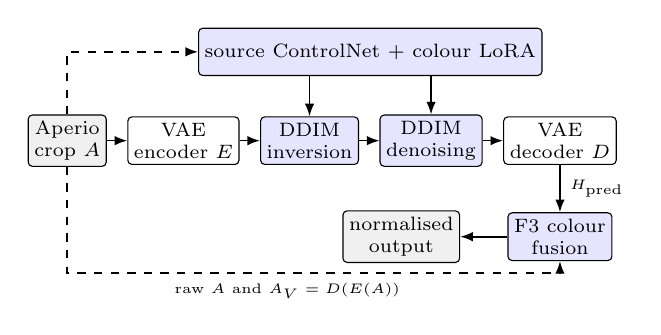
\begin{tikzpicture}[
  node distance=3.2mm and 2.6mm,
  box/.style={draw, rounded corners=1.5pt, align=center, font=\scriptsize, inner sep=2.2pt, minimum height=6mm},
  io/.style={box, fill=gray!12},
  ours/.style={box, fill=blue!10},
  arr/.style={-{Latex[length=1.6mm]}, semithick}]
\node[io] (a) {Aperio\\crop $A$};
\node[box, right=of a] (e) {VAE\\encoder $E$};
\node[ours, right=of e] (inv) {DDIM\\inversion};
\node[ours, right=of inv] (fwd) {DDIM\\denoising};
\node[box, right=of fwd] (d) {VAE\\decoder $D$};
\path (inv.north) -- (fwd.north) coordinate[midway] (mid);
\node[ours, above=5mm of mid] (cn) {source ControlNet + colour LoRA};
\node[ours, below=6mm of d] (f3) {F3 colour\\fusion};
\node[io, left=6mm of f3] (out) {normalised\\output};
\draw[arr] (a) -- (e);
\draw[arr] (e) -- (inv);
\draw[arr] (inv) -- (fwd);
\draw[arr] (fwd) -- (d);
\draw[arr] (cn.south -| inv.north) -- (inv.north);
\draw[arr] (cn.south -| fwd.north) -- (fwd.north);
\draw[arr, dashed] (a.north) |- (cn.west);
\draw[arr] (d) -- node[right, font=\tiny]{$H_{\mathrm{pred}}$} (f3);
\draw[arr] (f3) -- (out);
\draw[arr, dashed] (a.south) |- node[pos=0.75, below, font=\tiny]{raw $A$ and $A_V=D(E(A))$} ([yshift=-1.5mm]f3.south west) -- ([yshift=-1.5mm]f3.south west -| f3.south) -- (f3.south);
\end{tikzpicture}
\caption{Final SD\,1.5 pipeline. The source conditions the ControlNet during inversion and denoising
(dashed), and the untouched source supplies fine structure to the F3 fusion. Shaded blue: components
trained or added in this work; the SD\,1.5 U-Net and VAE encoder stay frozen.}
\label{fig:pipeline}
\end{figure}

\subsection{The VAE ceiling, fusion and decoder fine-tuning}
Every diffusion output is decoded by the VAE, which compresses a 512$\times$512$\times$3 crop 48$\times$
into a 64$\times$64$\times$4 latent. We measure the ceiling this imposes by self-reconstruction,
$\mathrm{SSIM}(x, D(E(x)))$ with a deterministic encode, and test three ways around it.

\textbf{Decoder swap.} The pretrained \texttt{sd-vae-ft-mse} decoder shares the stock encoder bit for bit,
so it decodes the same latents without retraining anything upstream.

\textbf{Detail fusion.} Instead of accepting the VAE-resynthesised image, we move only the learned
colour change back onto the untouched source. All arithmetic is in floating-point CIELAB; we write
$X=(L_X,a_X,b_X)$ for an image in LAB, $H=H_{\mathrm{pred}}$ for the translated prediction and $G_\sigma$ for
a Gaussian blur of width $\sigma$ pixels. Three variants were compared. F1 keeps the source luminance and
takes chroma from the prediction,
\begin{equation}
F_1=(L_A,\;a_H,\;b_H).
\label{eq:f1}
\end{equation}
F2 keeps the prediction's low-frequency luminance and re-injects the source's high-frequency detail,
\begin{equation}
F_2=\bigl(G_\sigma(L_H)+\alpha\,[L_A-G_\sigma(L_A)],\;a_H,\;b_H\bigr).
\label{eq:f2}
\end{equation}
F3 transfers all three channels, but only as a smoothed residual measured against the model's own
reconstruction of the source, $A_V=D(E(A))$:
\begin{equation}
F_3=A+\beta\,G_\sigma\!\bigl(H-A_V\bigr).
\label{eq:f3}
\end{equation}
Each term of Eq.~\eqref{eq:f3} has one job. Subtracting $A_V$ cancels what the VAE does to every image
(its blur and colour offset), so $H-A_V$ approximates the scanner shift alone; $G_\sigma$ removes
high-frequency texture that the generator invented; and $\beta$ sets how much of the shift is applied.
Because the added residual is smooth, F3 can change only low-frequency colour, and the fine structure of
$F_3$ is that of $A$ by construction. Variant and parameters were chosen on internal training-domain crops
and frozen ($\sigma=8$, $\beta=0.5$) before any held-out run. The real Hamamatsu image is never read to
construct a fused output; one construction bug that briefly did so (it produced SSIM $\approx0.998$) was
caught, and the corrected run was checked against the raw source.

\textbf{Decoder fine-tune.} With the encoder frozen, so that the latent space and every trained component
remain valid, we fine-tune only the decoder (49.5M parameters, initialised from \texttt{ft-mse}) on about
2{,}700 non-held-out H\&E patches (MITOS slides of both scanners, TCGA, PanNuke and the A03/H03 crops)
with an L1 + 0.3\,LPIPS~\citep{zhang2018lpips} loss for 3{,}000 steps. Checkpoints are selected on whole
non-held-out validation slides.

\subsection{Baselines}
\label{sec:baselines}
Three classical normalisers (Macenko, Reinhard, histogram matching) use one reference image each. Three
learned normalisers are trained on exactly the same 50 A03/H03 pairs as the colour LoRA, so every trained
method has the same data budget. StainNet~\citep{kang2021stainnet} is a three-layer 1$\times$1 convolutional
colour map (1{,}283 parameters) trained with a paired L1 loss; ParamNet~\citep{kang2024paramnet} uses a
ResNet18 to predict the weights of a per-image 1$\times$1 colour map, trained with its CycleGAN-style recipe;
StainGAN~\citep{shaban2019staingan} is a standard CycleGAN~\citep{zhu2017cyclegan} (ResNet-9 generator,
PatchGAN discriminator), trained here because its authors released no weights. Public MITOS-trained
checkpoints were deliberately not used, because their training splits are unknown and could include our
held-out slides. All baselines use final-step weights (no held-out checkpoint selection) and are scored by
the same crop and registration pipeline as the diffusion methods.

\subsection{SDXL transfer and exploratory probes}
The best SD\,1.5 design is ported to SDXL~\citep{podell2023sdxl} with its own rank-8 LoRA, a
source-conditioned ControlNet and an fp32 VAE (SDXL's VAE produces NaNs in fp16), at 512\,px and natively at
1024\,px, without repeating the ablation ladder. Because the 1024\,px model is data-starved at 50 pairs, two
supplementary runs use 96 non-overlapping and 144 overlapping crop pairs from the same A03/H03 frames.

Two newer backbones were probed for feasibility only. SD\,3.5-large, a transformer-based latent model with a
16-channel VAE, was tested for LoRA training cost and colour transfer. PixCell, a 0.6B-parameter
histopathology diffusion transformer that uses the same 16-channel VAE and is conditioned on a single UNI2-h
image embedding rather than text, was tested for cost, reconstruction ceiling and zero-fine-tuning
generation. PixCell is outside the proposal's scope and is reported as exploration only.

\section{Results}
\label{sec:results}

Table~\ref{tab:main} gathers every \AtoH{} configuration on the held-out set. Where we quote a recovery
$\dlab$ below, it is $W_{\mathrm{LAB}}(\text{raw},\text{target})-W_{\mathrm{LAB}}(\text{output},\text{target})$
on the slide in question, so positive means closer to the real scanner than doing nothing.

\begin{table*}[t]
\centering
\caption{\AtoH{} results on the five held-out slides. LAB Wasserstein (Eq.~\ref{eq:wlab}, lower is
better) and SSIM against the registered Hamamatsu scan; \emph{typical} is A08, A09, A13 and A16. Every
trained method uses the same 50 A03/H03 pairs. Rows marked $^\dagger$ average three seeds (1{,}488
crop-seeds); the rest use one (496 crops). The raw row is computed over the full baseline crop set.
Bold: best normaliser per column.}
\label{tab:main}
\small
\begin{tabular}{llrrrrrr}
\toprule
& & \multicolumn{3}{c}{LAB Wasserstein $\downarrow$} & \multicolumn{3}{c}{SSIM $\uparrow$}\\
\cmidrule(lr){3-5}\cmidrule(lr){6-8}
Group & Method & ALL & typical & A06 & ALL & typical & A06\\
\midrule
Reference & Raw Aperio (no normalisation) & 33.83 & 25.41 & 94.84 & 0.733 & 0.748 & 0.627\\
\midrule
Classical & Macenko~\cite{macenko2009normalisation} & 24.80 & 21.02 & 50.30 & 0.628 & 0.649 & 0.479\\
 & Reinhard~\cite{reinhard2001colortransfer} & 28.02 & 26.79 & 36.34 & 0.681 & 0.701 & 0.545\\
 & Histogram matching & 30.61 & 31.33 & \textbf{25.72} & 0.651 & 0.664 & 0.562\\
\midrule
Learned & StainNet~\cite{kang2021stainnet} & 55.51 & 58.02 & 38.58 & 0.512 & 0.518 & 0.471\\
 & ParamNet~\cite{kang2024paramnet} & 17.27 & \textbf{8.55} & 76.15 & 0.753 & 0.769 & 0.644\\
 & StainGAN~\cite{shaban2019staingan} & \textbf{15.66} & 13.55 & 29.92 & \textbf{0.764} & \textbf{0.772} & \textbf{0.709}\\
\midrule
SD\,1.5 ladder & A0 frozen img2img & 32.89 & 23.65 & 95.22 & 0.285 & 0.299 & 0.186\\
 & A1 + ControlNet (Canny) & 33.10 & 23.88 & 95.35 & 0.389 & 0.408 & 0.260\\
 & A2 + colour LoRA (rank 8) & 32.12 & 22.96 & 93.92 & 0.289 & 0.304 & 0.191\\
 & A3 ControlNet + LoRA & 32.52 & 23.35 & 94.39 & 0.386 & 0.404 & 0.259\\
 & A4 + LCM-LoRA (8 steps) & 33.96 & 24.91 & 95.06 & 0.398 & 0.417 & 0.272\\
 & A5 + histopathology warm-start & 33.96 & 25.29 & 92.46 & 0.389 & 0.407 & 0.265\\
\midrule
This work & Source ControlNet + LoRA, img2img$^\dagger$ & 30.95 & 22.11 & 90.64 & 0.448 & 0.470 & 0.307\\
 & + DDIM inversion$^\dagger$ & 25.10 & 17.98 & 73.12 & 0.496 & 0.514 & 0.373\\
 & + \texttt{ft-mse} decoder$^\dagger$ & 24.53 & 16.86 & 76.32 & 0.557 & 0.574 & 0.438\\
 & + fine-tuned decoder$^\dagger$ & 25.86 & 17.95 & 79.23 & 0.616 & 0.634 & 0.498\\
 & DDIM inversion + F3 fusion & 26.56 & 18.11 & 83.59 & 0.729 & 0.746 & 0.617\\
\bottomrule
\end{tabular}
\end{table*}

\subsection{The ablation ladder}
No rung of the ladder comes close to the classical baselines (Fig.~\ref{fig:ladder}). The colour LoRA (A2) recovers only
$\dlab=+1.72$ pooled, and on typical slides its LAB distance falls from 25.41 to 22.96. ControlNet raises
SSIM by about 0.10 (A0 0.285 to A1 0.389) but does not move colour. LCM-LoRA (A4) and the histopathology
warm-start (A5) cancel the small colour gain. Ranks 4 and 8 differ by only 0.1--0.3 in LAB distance.
Sweeps show why denoising strength is a poor control knob: with 8 LCM steps, strengths 0.50 and 0.60 give
byte-identical outputs, because the number of steps actually run is $\lfloor 8s\rfloor$. Larger strengths
help the outlier A06 (A5 reaches $\dlab=+24.4$ at 0.70) but damage typical slides (A08 $-7.0$), so no
single strength is usable.

\begin{figure}[t]
\centering
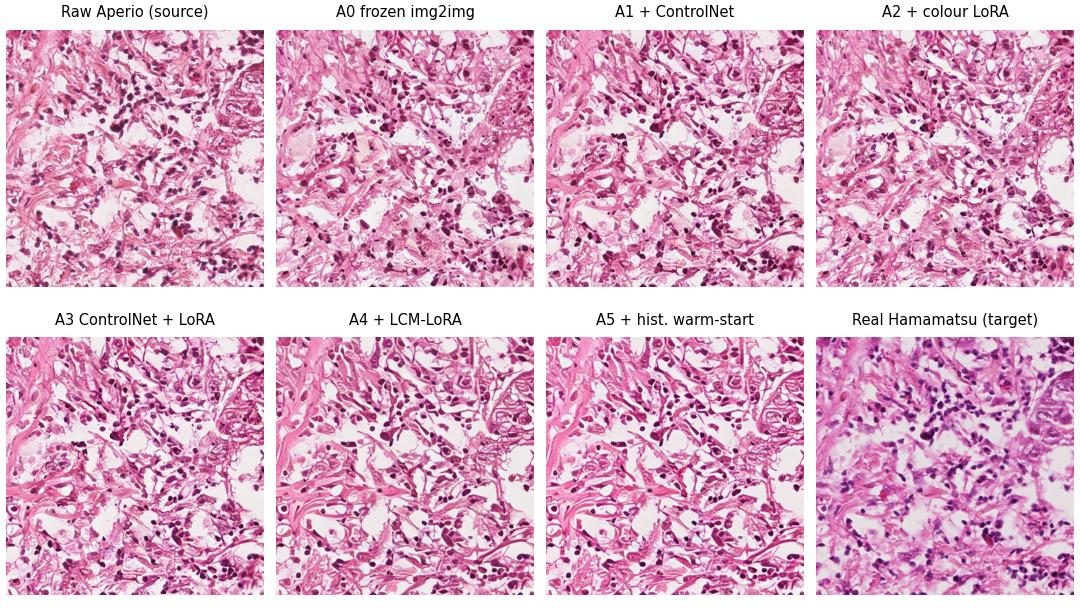
\includegraphics[width=\columnwidth]{ladder_grid_a08.jpg}
\caption{The A0--A5 ladder on a held-out A08 crop (strength 0.30) with the Aperio source and the real
Hamamatsu target. Every rung keeps the source's pink cast; none reaches the target's purple.}
\label{fig:ladder}
\end{figure}

\subsection{Source conditioning and DDIM inversion}
Conditioning on the source image gives a real but modest gain over the ladder ($\dlab=+2.89$, SSIM 0.448).
Replacing random img2img noise with DDIM inversion is the largest single improvement: LAB distance falls to
25.10 pooled and 17.98 on typical slides, every held-out slide moves towards the target (A06 recovery
$+21.7$), and SSIM rises to 0.496. In the reverse direction (\HtoA) the same model fails
($\dlab=-15.6$, a magenta drift), so the gain is direction-dependent.

\subsection{The VAE ceiling}
\label{sec:vae}
SSIM stays far below the raw scan's 0.733 for every diffusion output because the VAE alone cannot
reproduce its input. Self-reconstruction SSIM on the held-out Aperio crops is 0.576 for the stock decoder,
0.618 for \texttt{ft-mse} and 0.646 for our fine-tuned decoder (Fig.~\ref{fig:vaebb}); on Hamamatsu crops it
is 0.726, 0.757 and 0.779, and the fine-tune is highest on every slide (Fig.~\ref{fig:app-vae}). It improves
100\% of Aperio crops, but the limit is generalisation rather than the frozen latent: the same decoder
trained on 16 crops reconstructs those crops at SSIM 0.88. Across backbones the ceiling tracks latent
capacity: SDXL's four-channel VAE reconstructs at only 0.492, while the 16-channel VAE shared by SD\,3.5 and
PixCell reaches 0.773 (eight A06 crops each, so these two are indicative only).

\begin{figure}[t]
\centering
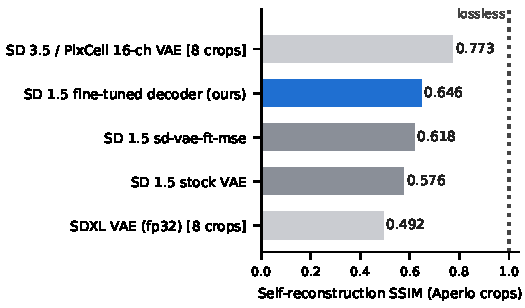
\includegraphics[width=\columnwidth]{vae_backbones.pdf}
\caption{VAE self-reconstruction SSIM, $\mathrm{SSIM}(x, D(E(x)))$, on held-out Aperio crops, across the
backbones used in this work. SD\,1.5 rows use all 496 crops; the SDXL and 16-channel rows use eight A06
crops. Every VAE stays well below the lossless value of 1.0 (dotted).}
\label{fig:vaebb}
\end{figure}

Decoding the DDIM-inversion latents with the better decoders raises translated SSIM from 0.496 to 0.557
(\texttt{ft-mse}) and 0.616 (fine-tuned), winning on every crop-seed. The fine-tune costs colour, though:
typical-slide LAB distance rises from 16.86 to 17.95 and A06 worsens to 79.2. Visual inspection explains
part of the SSIM gain. On two inspected crops the fine-tuned decoder keeps only 21--30\% of the input's
fine-detail energy (Laplacian variance), against 52--59\% for \texttt{ft-mse}, and shifts the blue channel
by 3--5 levels. The real Hamamatsu scans are themselves soft, at 18--24\% of the Aperio source's detail,
so much of the translated SSIM gain comes from matching the target scanner's softness rather than from
recovering structure.

\subsection{Detail fusion}
\textbf{Choosing the variant.} Table~\ref{tab:fusion} compares the three fusion rules and the F3
parameters on internal training-domain crops. These crops are coordinate-corresponding rather than
registered, so absolute SSIM is low and only comparisons within the table are meaningful. Every variant
raises SSIM over the unfused prediction. F1 is worse than F3 on both axes; pasting the prediction's
unblurred chroma onto the source luminance is the likely cause. F2 sits at other points of the trade-off:
more SSIM for much worse colour ($\alpha=0.5$), or the lowest LAB distance at lower SSIM ($\alpha=1$). F3
was chosen as the best balance, and on visual inspection it was indistinguishable from the source in
nuclear boundaries and chromatin, with no haloes, ringing or gamut clipping.

\textbf{What the sweep shows.} SSIM is flat across $\beta$, from $0.10$ to $1.00$, and nearly flat across
$\sigma$ once $\sigma\geq8$. This is the mechanism of Eq.~\eqref{eq:f3} at work: the blurred residual
cannot reach fine structure at any strength, so the structural gain comes from starting at the source
pixels at all. Colour traces a U-shape in $\beta$ with its minimum at 0.5. Small $\beta$ leaves the source
colour almost unchanged, and large $\beta$ adds more of a \emph{smoothed approximation} of the prediction's
shift, which is worse than the shift itself.

\begin{table}[t]
\centering
\caption{Fusion design on internal training-domain crops (SSIM, and LAB Wasserstein against the paired
Hamamatsu crop). Top: the three rules on 50 crops. Bottom: the F3 parameter sweep on 20 crops. Bold: the
frozen configuration.}
\label{tab:fusion}
\footnotesize
\begin{tabular}{llrr}
\toprule
& Configuration & SSIM $\uparrow$ & LAB W. $\downarrow$\\
\midrule
\multicolumn{4}{l}{\emph{Fusion rules, 50 crops}}\\
& Unfused DDIM-inversion prediction & 0.1604 & 22.11\\
& F1, source luminance (Eq.~\ref{eq:f1}) & 0.1826 & 24.63\\
& F2, $\alpha=0.5$ (Eq.~\ref{eq:f2}) & 0.1955 & 30.74\\
& F2, $\alpha=1.0$ & 0.1813 & 20.30\\
& \textbf{F3, $\sigma=8$, $\beta=0.5$} (Eq.~\ref{eq:f3}) & \textbf{0.1854} & \textbf{22.67}\\
\midrule
\multicolumn{4}{l}{\emph{F3 sweep, 20 crops (unfused: 0.1644 / 21.46)}}\\
& $\sigma=8$, $\beta=0.10$ & 0.1866 & 25.63\\
& $\sigma=8$, $\beta=0.25$ & 0.1866 & 23.95\\
& \textbf{$\sigma=8$, $\beta=0.50$} & \textbf{0.1866} & \textbf{21.44}\\
& $\sigma=8$, $\beta=0.75$ & 0.187 & 21.75\\
& $\sigma=8$, $\beta=1.00$ & 0.1865 & 22.50\\
& $\sigma=4$, $\beta=0.75$ & 0.185 & 21.74\\
& $\sigma=16$, $\beta=0.75$ & 0.187 & 21.75\\
\bottomrule
\end{tabular}
\end{table}

\textbf{Held-out result.} Fusing only the learned colour change onto the raw source raises SSIM to 0.729 pooled
and 0.746 on typical slides, above every classical baseline, while keeping most of the colour shift:
typical-slide LAB distance is 18.11 (raw 25.41) and windowed LAB 18.65, closer to the target than Macenko
(21.88), Reinhard (27.42) or histogram matching (31.90). Fig.~\ref{fig:f3} shows the process. A06 benefits
least (LAB 83.6) and stays visibly paler than the Hamamatsu scan. Fusion also absorbs other structural
gains: a three-member self-ensemble raises unfused SSIM from 0.496 to 0.543 but adds nothing after fusion
(0.7288 against 0.7290), and the fine-tuned decoder adds nothing either (0.7289) while worsening fused
windowed LAB from 27.08 to 27.74. In the failed \HtoA{} direction, fusion applied unchanged raises SSIM from
0.548 to 0.730 and shrinks the colour loss from $\dlab=-15.6$ to $-5.3$, although colour is still worse
than doing nothing. It also transfers to SDXL with the same frozen parameters (Table~\ref{tab:sdxl}).

\begin{figure*}[t]
\centering
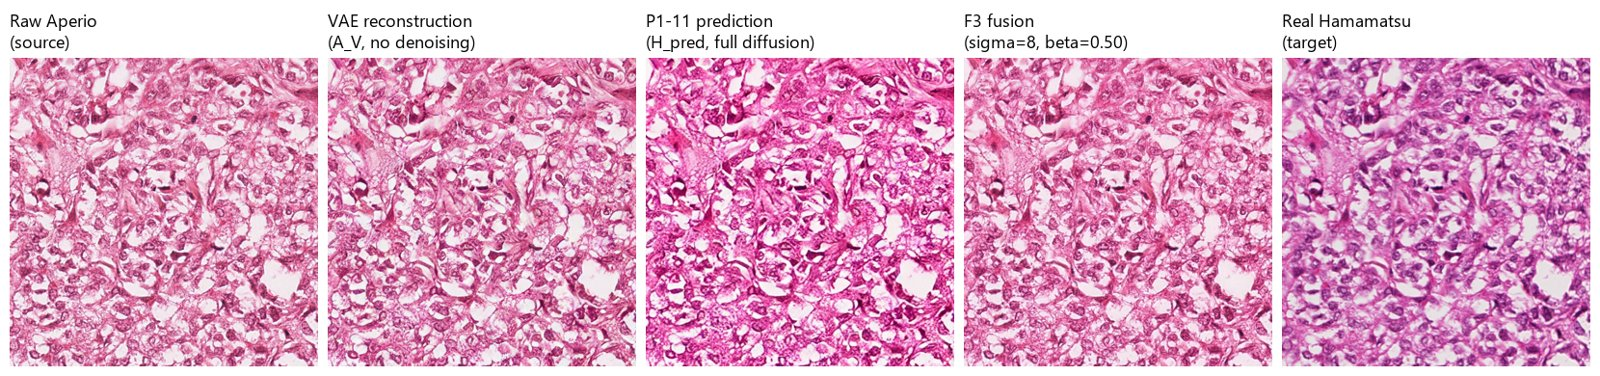
\includegraphics[width=\textwidth]{p1_16_a08.jpg}
\caption{F3 fusion on held-out slide A08: raw Aperio source $A$, its VAE reconstruction $A_V$, the
DDIM-inversion prediction $H_{\mathrm{pred}}$, the fused output (Eq.~\ref{eq:f3}, $\sigma=8$, $\beta=0.5$)
and the registered real Hamamatsu target.}
\label{fig:f3}
\end{figure*}

\subsection{Learned baselines}
Trained on the same 50 pairs, ParamNet and StainGAN outperform every diffusion configuration in
Table~\ref{tab:main} (Fig.~\ref{fig:compare}). ParamNet has the lowest typical-slide LAB distance (8.55) and StainGAN the lowest
pooled distance (15.66) and the highest SSIM (0.764 pooled, 0.709 on A06), above even the raw scan's
pixel similarity. StainNet, a per-pixel 1$\times$1 network with 1{,}283 parameters, is worse than doing
nothing on every typical slide; a 150{,}000-step retrain plateaued at the same training loss, so this is a
capacity limit, not under-training. The ranking holds in the \HtoA{} direction: on typical slides ParamNet
recovers $\dlab=+17.28$ and StainGAN $+10.75$, while StainNet loses $-28.38$. The classical methods only
beat the raw input pooled because of A06: on typical \AtoH{} slides Reinhard ($-1.38$) and histogram
matching ($-5.92$) are slightly worse than doing nothing, and only Macenko gains ($+4.39$). ParamNet is also
the most consistent learned method across the four typical slides ($+9.8$ to $+19.1$ in \AtoH{}).

\begin{figure*}[t]
\centering
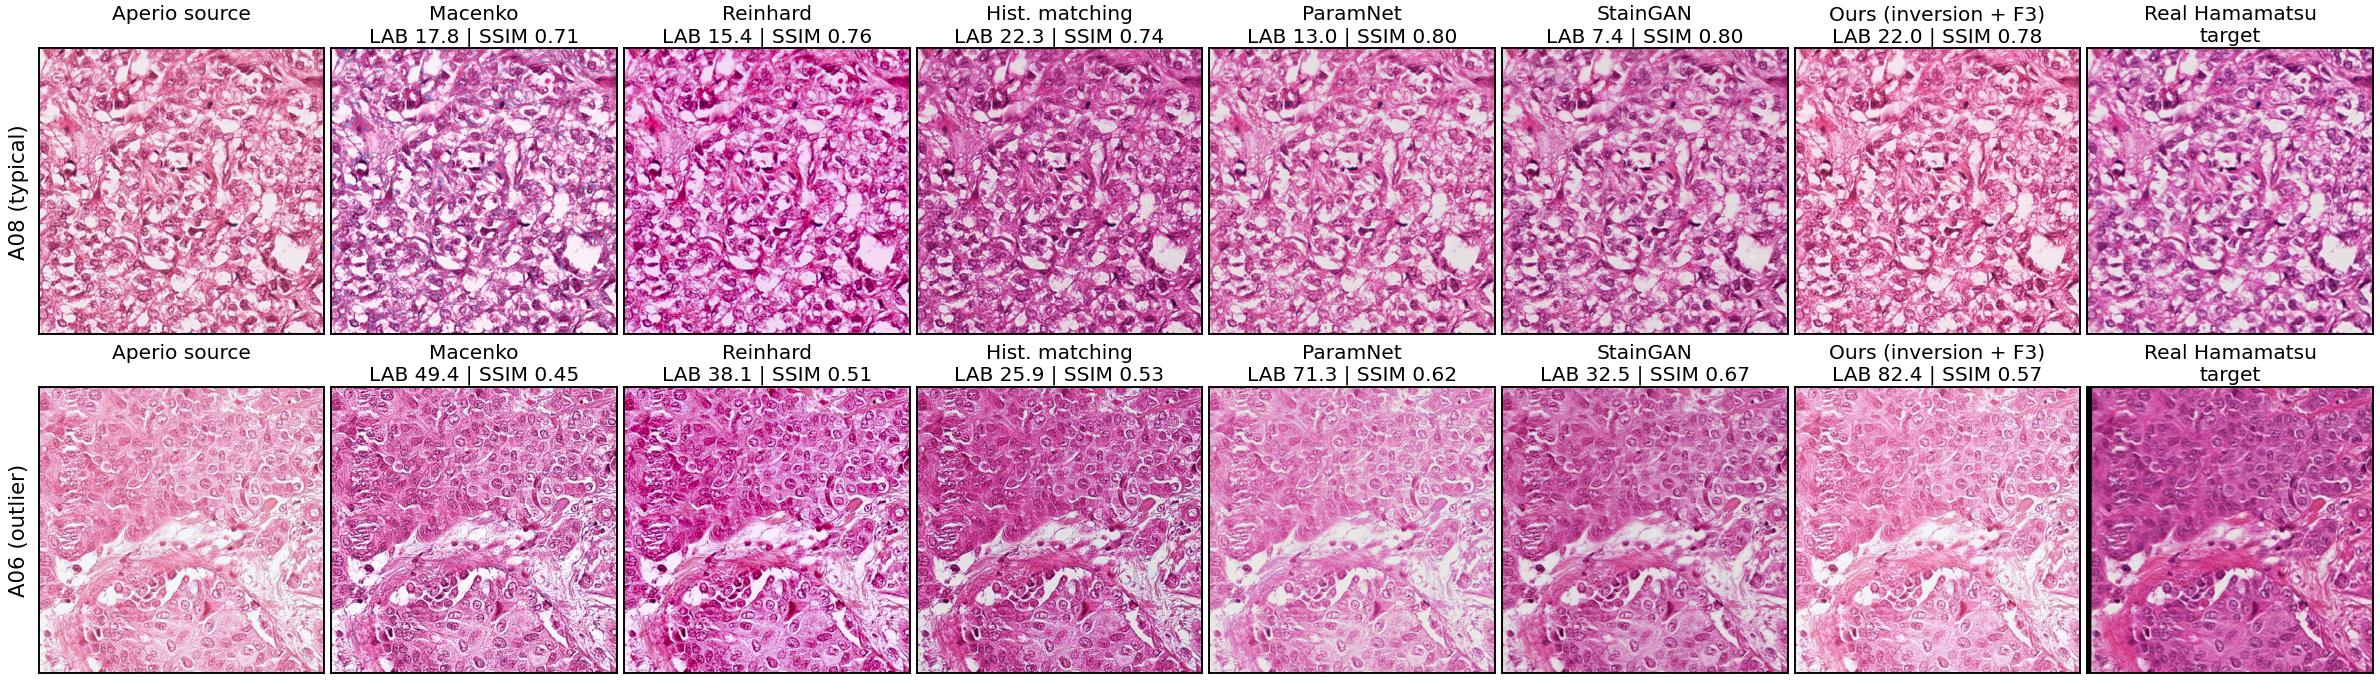
\includegraphics[width=\textwidth]{normaliser_comparison.jpg}
\caption{One held-out crop each from A08 (typical) and A06 (outlier), normalised by every method, with the
per-crop LAB Wasserstein and SSIM against the registered target. These are single crops, not averages:
on this A08 crop our fused output (LAB 22.0) is weaker than its typical-slide mean (18.1). On A06,
ParamNet and our output stay visibly paler than the target, while histogram matching, StainGAN and
Reinhard come closer.}
\label{fig:compare}
\end{figure*}

\begin{table}[t]
\centering
\caption{Structural safety: Relative Dice of HoVer-Net nuclei on 130 Lizard images (95\% bootstrap CI).
Pass threshold 0.95. ``Ours'' is the final pipeline (DDIM inversion + F3 fusion); ``A4-type'' is the
earlier colour LoRA + ControlNet + LCM operating point (strength 0.20).}
\label{tab:reldice}
\small
\begin{tabular}{lrl}
\toprule
Normaliser & Relative Dice & 95\% CI\\
\midrule
ParamNet & \textbf{0.999} & [0.996, 1.001]\\
Ours: inversion + F3 & \textbf{0.994} & [0.992, 0.997]\\
Reinhard & 0.923 & [0.905, 0.939]\\
Diffusion: inversion only & 0.893 & [0.886, 0.900]\\
Diffusion (A4-type) & 0.875 & [0.867, 0.882]\\
Histogram matching & 0.793 & [0.763, 0.822]\\
Macenko & 0.737 & [0.684, 0.787]\\
StainGAN & 0.724 & [0.692, 0.756]\\
StainNet & 0.622 & [0.567, 0.675]\\
\bottomrule
\end{tabular}
\end{table}

\subsection{Structural safety and unseen centres}
Two normalisers pass the Relative Dice gate (Table~\ref{tab:reldice}): ParamNet and our final pipeline
(0.994, 95\% CI $[0.992, 0.997]$, entirely above 0.95). The pass comes from fusion, not from the diffusion
output itself: the unfused inversion output fails at 0.893, and fusion raises Dice on 129 of the 130 images
(mean $+0.071$). This is expected from Eq.~\eqref{eq:f3}, which keeps the source's high frequencies and adds
only a blurred colour change, so nucleus boundaries come from the source. The secondary metrics agree: against
the original images, the fused output keeps IoU (0.535 against 0.539), object-level F1 (0.738 against 0.733) and
the predicted-to-true nucleus count ratio (0.686 against 0.668), while StainGAN lowers object F1 to 0.503 and
the count ratio to 0.384. The earlier A4-type operating point
loses 12.5\% of HoVer-Net's agreement with the ground truth, and StainGAN, despite its high SSIM, loses 28\%,
which is consistent with GANs altering nuclei. On CAMELYON17~\cite{bandi2018camelyon17}, measured as the
mean pairwise LAB distance $D$ between five hospital centres (2{,}103 patches, $D_{\mathrm{pre}}=56.70$), no
SD\,1.5 configuration brings the centres closer. The final pipeline is neutral with fusion
($\Delta D=+0.14$, 95\% bootstrap CI $[-0.22, 0.51]$, 4 of 10 centre pairs improved) and worse without it
($+1.29$ $[0.24, 2.49]$, 3 of 10), as is the A4-type operating point ($+0.83$ $[0.44, 1.19]$, 1 of 10). The CIs
resample the 10 centre pairs, which share centres, so they are supportive only.

\subsection{Downstream clinical utility}
The planned clinical test, an atypia classifier trained on Aperio and scored on normalised Hamamatsu
frames, produced no valid evidence in either direction (Appendix~\ref{app:clinical}). An early result in
which diffusion beat every classical method had been scored in the wrong direction and is retracted. In the
corrected direction no configuration beats the raw input, including our fused pipeline (recovery 0.0, 95\%
CI $[-0.025, +0.025]$). Two rebuilt classifiers, a frozen UNI2-h probe and a criteria-supervised model,
then failed their own pre-registered validity gates, so no atypia number is used as evidence.

\subsection{Few-step inference}
Generic LCM-LoRA on the source-conditioned model is a speed--quality trade-off rather than a match: its best
setting (6 steps, guidance 2.0, strength 0.70) gives A06 SSIM 0.334 and $\dlab=+9.7$, against 0.373 and
$+21.7$ for 50-step DDIM inversion, and A08 0.515/$+3.0$ against 0.537/$+7.2$. Distilling a task-specific
LCM from the source-conditioned teacher was worse than the generic adapter under a pre-committed rule
(paired win rate 30 of 80 crops against 50 of 80).

\subsection{Portability to SDXL}
SDXL transfers the method only with source conditioning and more data than the few-shot budget
(Table~\ref{tab:sdxl}). The ladder configuration (A4) and its warm-started variant (A5) move colour away from
the target, despite SDXL's higher SSIM. Source conditioning works at 512\,px, but natively at 1024\,px the
50-pair model is data-starved: it recovers less colour than doing nothing on every slide, and diagnostics show
that removing its LoRA makes colour worse still, so the adapter helps but is too weak. With 96 or 144 pairs
recovery turns positive, but each extra $\sim$48 pairs adds only about 0.1 in $\dlab$. A source ablation on
the 144-pair model (SSIM 0.318 correct, 0.114 shuffled, 0.109 zero) confirms that it uses the source. F3
fusion transfers unchanged (SSIM 0.732), and with the 144-pair model SDXL passes the CAMELYON17 test with a
small effect ($D_{\mathrm{post}}=54.32$ against $D_{\mathrm{pre}}=56.67$, $\Delta D=-2.35$ $[-2.97, -1.57]$,
9 of 10 centre pairs closer; $-0.67$ $[-0.96, -0.34]$, 8 of 10, with F3 fusion). In
the \HtoA{} direction, where SD\,1.5 fails ($\dlab=-15.6$), SDXL succeeds at both resolutions. Fig.~\ref{fig:sdxl}
shows one crop across the SDXL configurations.

\begin{table}[t]
\centering
\caption{SDXL held-out results (\AtoH{} unless stated; LAB Wasserstein and SSIM as in Table~\ref{tab:main};
source-conditioned rows average three seeds, about 1{,}485 crop-seeds). The 96- and 144-pair runs exceed
the 50-pair budget and are supplementary.}
\label{tab:sdxl}
\footnotesize
\setlength{\tabcolsep}{2.5pt}
\begin{tabular}{lrrrrr}
\toprule
& \multicolumn{3}{c}{LAB W. $\downarrow$} & \multicolumn{2}{c}{SSIM $\uparrow$}\\
\cmidrule(lr){2-4}\cmidrule(lr){5-6}
Configuration & ALL & typ. & A06 & ALL & A06\\
\midrule
Raw Aperio & 33.83 & 25.41 & 94.84 & 0.733 & 0.627\\
A4, strength 0.20 & 39.44 & 30.70 & 98.42 & 0.527 & 0.386\\
A5 warm-start, 0.20 & 39.14 & 30.36 & 98.40 & 0.526 & 0.385\\
Source-cond., 512\,px, 50 pairs & 32.62 & 23.81 & 92.14 & 0.392 & 0.257\\
Source-cond., 1024\,px, 50 pairs & 39.43 & 30.85 & 98.32 & 0.431 & 0.313\\
\quad 96 pairs & 32.51 & 23.79 & 92.29 & 0.442 & 0.322\\
\quad 144 overlapping pairs & 32.40 & 23.80 & 91.42 & 0.446 & 0.335\\
\quad 144 pairs + F3 fusion & 31.78 & 23.06 & 91.62 & 0.732 & 0.638\\
\midrule
\HtoA{}, 512\,px & 24.90 & 17.33 & 75.99 & 0.355 & 0.239\\
\HtoA{}, 1024\,px & 25.17 & 16.68 & 82.47 & 0.386 & 0.274\\
\bottomrule
\end{tabular}
\end{table}

\begin{figure*}[t]
\centering
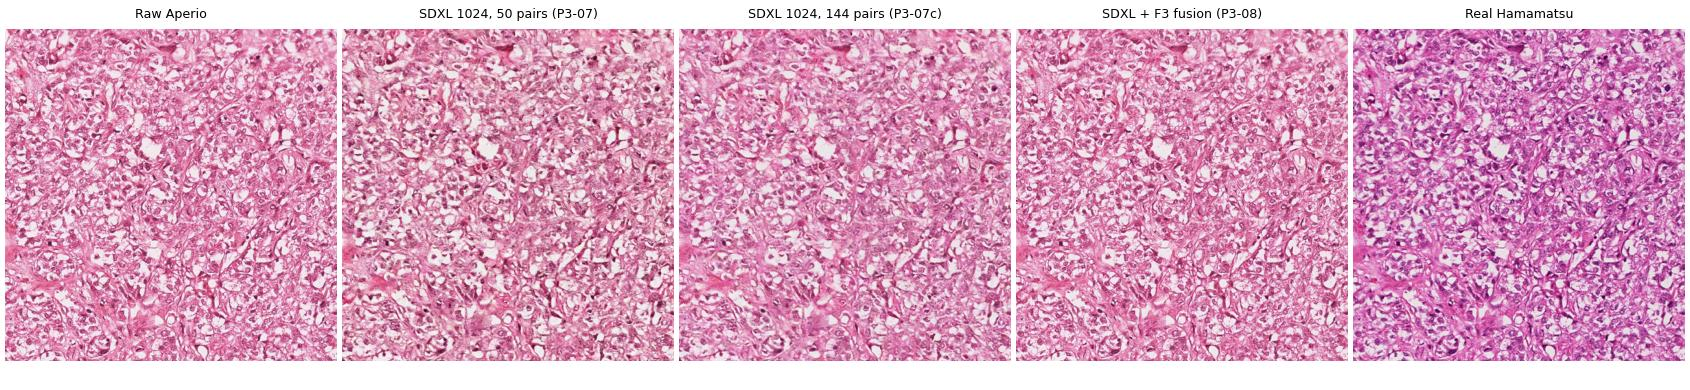
\includegraphics[width=\textwidth]{sdxl_panel_a08.jpg}
\caption{SDXL at native 1024\,px on one held-out A08 crop (frame 00A, origin (0,0), seed 0): raw Aperio,
the 50-pair and 144-pair source-conditioned models, the 144-pair model with F3 fusion, and the registered real
Hamamatsu target. All SDXL outputs stay close to the Aperio colour.}
\label{fig:sdxl}
\end{figure*}

\subsection{Newer backbones (exploratory probes)}
Both newer backbones are feasible to adapt but not yet useful (Table~\ref{tab:cost}). An SD\,3.5-large
rank-8 LoRA trains in about five times SD\,1.5's time and fits a 24\,GB GPU. On 20 A06 crops at 1024\,px
(strength 0.30, without the T5 text encoder to save memory) it recovers $\dlab=+4.77$ but reaches only SSIM
0.183, far below SD\,1.5 and SDXL; because this covers only the outlier slide it is not a general result.
PixCell is the cheapest backbone to adapt and its 16-channel VAE has the highest reconstruction ceiling
(0.773, Fig.~\ref{fig:vaebb}). But generation from a crop's own UNI2-h embedding, without fine-tuning,
scores SSIM 0.045 against the registered target and 0.036 against its own source: a single global embedding
carries no information about where nuclei are (Fig.~\ref{fig:app-pixcell}). Using it for normalisation would
need a source-image conditioning branch for a diffusion transformer, which was not built.

\begin{table}[t]
\centering
\caption{Cost of a rank-8 LoRA, 1{,}000 steps, on one RTX~3090 (exploratory probes).}
\label{tab:cost}
\footnotesize
\begin{tabular}{lrrr}
\toprule
& SD\,1.5 & SD\,3.5-large & PixCell\\
\midrule
Wall-clock (s) & 160.5 & 798.8 & \textbf{130.3}\\
Peak VRAM (GB) & -- & 17.77 & \textbf{4.20}\\
Trainable parameters & 1.59M & 5.91M & 2.06M\\
\bottomrule
\end{tabular}
\end{table}

\section{Discussion}
\label{sec:discussion}

Table~\ref{tab:hyp} answers the four hypotheses the project committed to before any results.

\begin{table}[t]
\centering
\caption{Pre-registered hypotheses and outcomes (SD\,1.5 unless stated).}
\label{tab:hyp}
\footnotesize
\setlength{\tabcolsep}{3pt}
\begin{tabular}{p{0.9cm}p{3.0cm}p{3.6cm}}
\toprule
H & Claim & Outcome\\
\midrule
H1 & $\leq$50 pairs suffice to generalise to the five held-out slides &
\textbf{Supported for SD\,1.5} with source conditioning and DDIM inversion (every slide improves);
not for SDXL at 1024\,px, which needed 144 pairs.\\
\midrule
H2 & Colour improves over raw input and classical baselines, on MITOS and CAMELYON17 &
\textbf{Partly.} Beats raw everywhere and classical on typical slides; loses to Macenko on A06 and to
ParamNet/StainGAN everywhere; CAMELYON17 fails for every SD\,1.5 configuration, final pipeline
included, and passes narrowly for SDXL.\\
\midrule
H3 & Relative Dice $\geq 0.95$ &
\textbf{Supported with fusion}: 0.994 for inversion + F3; not without it (0.893 unfused, 0.875
for the A4-type point).\\
\midrule
H4 & 4-step LCM matches 50-step DDIM &
\textbf{Not supported}: generic LCM is 12.5$\times$ faster but loses quality; task-specific distillation
is worse.\\
\bottomrule
\end{tabular}
\end{table}

\textbf{Why the learned baselines win.} ParamNet and StainNet apply a colour map to the input pixels, and
StainGAN's CycleGAN generator keeps a wide feature map (a quarter of the resolution, hundreds of
channels); none of them passes the image through a 48$\times$ compressing four-channel latent. Every diffusion output is resynthesised by the VAE, which alone limits SSIM to
0.576--0.646 on Aperio crops (Section~\ref{sec:vae}). F3 fusion is, in effect, our way of turning the
diffusion model back into a colour map applied to the source: its success on structure and the
learned colour maps' success on colour point in the same direction. With 50 pairs, the strong image prior
of a diffusion model does not compensate for the information it loses in its own bottleneck.

\textbf{Colour metrics.} LAB Wasserstein compares colour histograms and ignores layout, so histogram
matching wins it on A06 by construction while scoring worse than doing nothing on typical slides. The
windowed variant and per-slide reporting were essential to avoid reading that as a real gain. Pixelwise
$\Delta E_{2000}$ tracks SSIM almost rank for rank, so it is not an independent colour check.

\textbf{Cost.} Timed on one RTX~3090 with loading excluded (Table~\ref{tab:app-speed}), the final pipeline
takes 6.27\,s per 512\,px crop, generic LCM at four steps 0.50\,s (12.5$\times$ faster), and SDXL 12.1\,s per
1024\,px crop, about 3.0\,s per 512\,px of tissue. The learned baselines take 2--25\,ms and the classical
ones 6--42\,ms. A 100{,}000$\times$100{,}000 pixel whole-slide image holds about 38{,}000 crops of
512\,px, so the final pipeline needs about 66 GPU-hours per slide, LCM 5.3 and SDXL 32, against
minutes for every baseline; the few-step LCM path that was meant to remove this cost did not hold its
quality (H4).

\textbf{Limitations.} All training data comes from one slide pair (A03/H03), so slide-level variation is
not represented in training. The learned baselines were trained once, with one seed each. Structural
safety rests on one segmenter (HoVer-Net) and one colon dataset (Lizard). The planned clinical-utility test has no valid
instrument: every atypia classifier we built failed its own pre-registered gate
(Appendix~\ref{app:clinical}), so no clinical-utility claim is made. The decoder smoothing analysis
rests on two inspected crops.

\textbf{Planned but not run.} Several planned items were not carried out and no result is claimed for
them: the mitosis-detection arm of the clinical-utility evaluation, which needs a separate object
detector; the SD\,3.5 probe's structural-ControlNet and SD\,3.5 Turbo few-step checks; a full-VAE fine-tune
with the LoRA and ControlNet retrained on its new latents (only the anchored version was run), and a cross-centre check of the fine-tuned decoder on CAMELYON17; and a
source-image conditioning branch for PixCell. Two choices also departed from the plan: the TCGA-BRCA colour
reference was not used as a secondary colour target, and the
attention-residual method~\cite{madusanka2025attentionresidual}, planned as the state-of-the-art colour
baseline, was not reproduced, so it is cited but not compared.

\section{Conclusion}
\label{sec:conclusion}

A frozen Stable Diffusion 1.5 model adapted from 50 coordinate-corresponding pairs can be made to normalise
between two scanners, but only after replacing the planned recipe. A target-only colour LoRA with
ControlNet and LCM barely moves colour. Source conditioning, DDIM inversion and a post-hoc fusion that
returns the learned colour change to the source pixels reach SSIM 0.729 and beat the classical baselines on
typical-slide colour. The VAE bottleneck explains most of the gap to the raw scan, and fine-tuning its
decoder raises SSIM mainly by smoothing. Learned nondiffusion baselines trained on the same 50 pairs
remain better on colour and SSIM. On nucleus preservation, ParamNet and the fused pipeline both pass the
Relative Dice test (0.999 and 0.994), and the unfused diffusion output does not. For
few-shot scanner normalisation, a well-chosen colour map currently beats a resynthesising generative
model; diffusion is most useful here as a source of colour change that fusion projects back onto the
original image.

\section*{Acknowledgment}
Computations were performed on the University of the Witwatersrand's mscluster
high-performance computing cluster. We thank the organisers of
MITOS-ATYPIA-14, CAMELYON17, Lizard, PanNuke and TCGA for making their data public.


\bibliographystyle{IEEEtran}
\bibliography{references}

\clearpage
\onecolumn
\appendices
\section{Additional results}
\label{app:results}

\subsection{Downstream clinical utility (atypia classifier)}
\label{app:clinical}

\textbf{Protocol.} The proposal's clinical-utility test trains a classifier on raw Aperio $\times$20 frames
of the eleven MITOS-ATYPIA-14 training slides to predict the adjudicated nuclear-atypia score (1--3), then
evaluates it on held-out Hamamatsu frames before and after normalisation. The recovery is the accuracy on
normalised frames minus the accuracy on raw Hamamatsu frames, so a positive value means normalisation
helped the classifier.

\textbf{A retracted result.} The first classifier (a ResNet18, \texttt{atypia\_r18}) appeared to favour
diffusion: the A3 rung at strength 0.50 gave a recovery of $+0.0625$, against $+0.0457$ for the best
classical method, Reinhard. A later audit found that every method had been run \AtoH{}, producing
Hamamatsu-styled images, whereas an Aperio-trained classifier needs \HtoA{} outputs. An A0 output was twice
as close in pixel error to its Aperio source as to its Hamamatsu reference, which confirmed the direction
error. The claim was retracted. Re-running in the correct direction, no configuration beats the raw input:
our source-conditioned \HtoA{} model gives $-0.025$ (CI crossing zero), and with F3 fusion the recovery is
exactly $0.0$ (95\% CI $[-0.025,+0.025]$, 120 frames), even though fusion raises its SSIM from 0.548 to
0.730. The rerun also found and fixed a second bug, in which the raw-Hamamatsu reference silently read
Aperio pixels.

\textbf{The classifier itself is not valid.} \texttt{atypia\_r18} predicts score 2 for about 91\% of held-out
frames even on raw Aperio, its own domain, where it scores 0.55 against 0.50 for always answering 2. Its
0.947 validation accuracy came from two slides containing 46 score-2 frames out of 47, so it is the
majority rate rather than skill. The labels are close to slide-determined: 19 of the 23 score-1 training
frames come from slide A12, and all 38 held-out score-1 frames come from A13 and A16. A retrained variant
with augmentation and class-balanced sampling was worse (raw-Hamamatsu accuracy 0.442 to 0.192).

\textbf{Two rebuilt classifiers, both gated.} Both use frozen UNI2-h features, nested leave-one-slide-out
cross-validation on the 297 training frames, and five pre-registered gates: balanced accuracy $>0.45$,
quadratic weighted kappa (QWK) $>0.2$, no class predicted for more than 80\% of frames, a slide-bootstrap
lower bound on balanced accuracy above chance ($1/3$), and non-zero recall for score 1 on the held-out-in-CV
slide A12. Table~\ref{tab:atypia} gives the results. The linear probe is at chance. Of three v2 candidates
(an ordinal head, attention-based multiple-instance pooling, and a two-stage model that first predicts the
x40 atypia criteria), the criteria model clears four of five gates but fails the bootstrap lower bound:
its interval $[0.26, 0.73]$ cannot be separated from chance with only eleven slides, and the threshold was
not relaxed afterwards. A separate within-slide test does pass. With each slide's mean removed from both
predictions and labels, so that recognising the slide cannot help, the predicted criteria correlate with
the rated ones (mean Spearman 0.240, CI $[0.148, 0.318]$; nuclei size 0.378, anisonucleosis 0.299,
nucleoli size 0.408, nuclei contour $-0.125$). Frozen features therefore carry real atypia signal, but not
yet enough for a valid score classifier. By protocol the held-out slides were never scored with these
models.

\begin{table}[!htbp]
\centering
\caption{Rebuilt atypia classifiers, nested leave-one-slide-out cross-validation on 297 training frames
(always predicting score 2 gives accuracy 0.747). Brackets: slide-bootstrap 95\% intervals.}
\label{tab:atypia}
\small
\begin{tabular}{lrrrcc}
\toprule
Model & Accuracy & Balanced accuracy & QWK & Recall (1 / 2 / 3) & Gates passed\\
\midrule
UNI2-h logistic probe & 0.579 & 0.312 [0.23, 0.46] & 0.022 & 0.00 / 0.73 / 0.21 & 1 of 5\\
v2 M1: ordinal head & 0.633 & 0.331 [0.27, 0.47] & 0.105 & 0.00 / 0.80 / 0.19 & 0 of 5\\
v2 M2: attention MIL & 0.478 & 0.292 [0.19, 0.50] & 0.098 & 0.00 / 0.57 / 0.31 & 1 of 5\\
v2 M3: criteria two-stage & 0.525 & 0.614 [0.26, 0.73] & 0.304 & 0.83 / 0.50 / 0.52 & 4 of 5\\
\bottomrule
\end{tabular}
\end{table}

\subsection{Other closed negatives}
\textbf{Differential diffusion.} To protect structure inside the diffusion process, each pixel was given
its own denoising strength from a Canny-derived change map, low near edges and high elsewhere. Six
configurations (dilation radius $\in\{2,4,8\}$, maximum strength $\in\{0.50,0.70\}$) gave SSIM 0.162--0.167
on 20 internal crops, against $0.162\pm0.006$ for the plain model, so there was no gain
(Fig.~\ref{fig:app-diffdiff}). On dense H\&E the protected and free regions interleave finely, and the
shared U-Net receptive field plausibly lets generation bleed into protected pixels. This failure is what
motivated fusion outside the U-Net.

\textbf{Round-trip consistency.} Translating A06 crops \AtoH{} and back to Aperio (50-step DDIM, strength
0.20) gives SSIM 0.143, PSNR 13.1\,dB and LAB distance 28.2 against the original
over 64 crops: the round trip does not return the input (Fig.~\ref{fig:app-roundtrip}).

\subsection{SDXL diagnostics and the decision gate}
\textbf{Decision gate.} At the end of Phase~1 the ladder configuration A4 was chosen as the base for SDXL,
and the A5 warm-start transfer was also run because A5 beat A4 on A06 by 2.6--8.7 in LAB distance, far above
the 0.1--0.3 run-to-run noise floor.

\textbf{Why native-1024 SDXL fails at 50 pairs.} Five diagnostics were run on the 50-pair 1024\,px model.
(D1) A baseline mismatch was ruled out: re-measured against a do-nothing baseline computed natively at
1024\,px, the model still gives $\dlab=-5.25$. (D2) Removing the LoRA makes colour worse ($-8.21$ against $-5.25$), so the LoRA helps by about 3
LAB but is too weak. (D3) RGB-only conditioning matches RGB plus Canny, and Canny alone collapses (SSIM 0.16,
$\dlab=-17.9$), so the edge channels are inert. (D4) No ControlNet scale gives positive recovery. (D5)
Raising the LoRA scale from 1.0 to 2.0 makes recovery monotonically worse ($-4.38$ to $-8.00$). The model is
data-starved, which the 96- and 144-pair runs confirm.

\textbf{The \AtoH{}/\HtoA{} asymmetry.} SD\,1.5 fails \HtoA{} while SDXL succeeds. Two diagnostics compared
the mean LAB of model outputs with the real scanner means (domain gap 17.97). Zero-source ControlNet
outputs refuted the idea that the asymmetry follows the backbone's default colour, because img2img leaks the
source colour into them. Pure text-to-image samples (Fig.~\ref{fig:app-t2i}) gave partial support (five of
six comparisons consistent), and SDXL at 1024\,px \HtoA{} remains an open counterexample: its default colour
leans the wrong way, yet it recovers $\dlab=+9.20$.

\clearpage

\section{Additional SD\,1.5 figures}
\label{app:sd15}

\begin{figure}[!htbp]
\centering
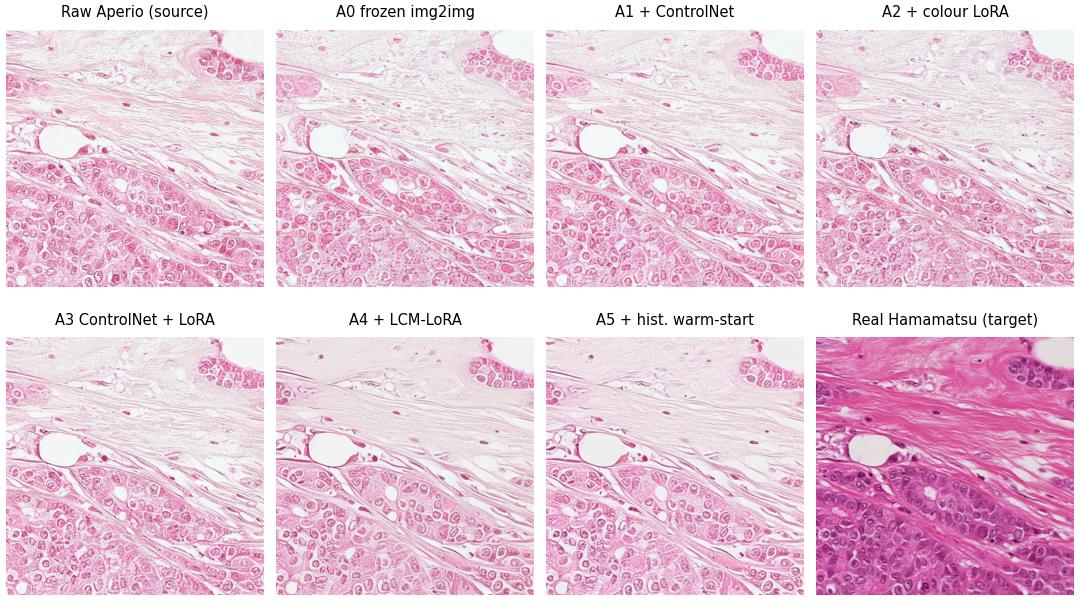
\includegraphics[width=0.62\textwidth]{ladder_grid_a06.jpg}
\caption{The A0--A5 ladder on the outlier slide A06 (strength 0.30). As on A08 (Fig.~\ref{fig:ladder}), no
rung approaches the target's colour.}
\label{fig:app-ladder}
\end{figure}

\begin{figure}[!htbp]
\centering
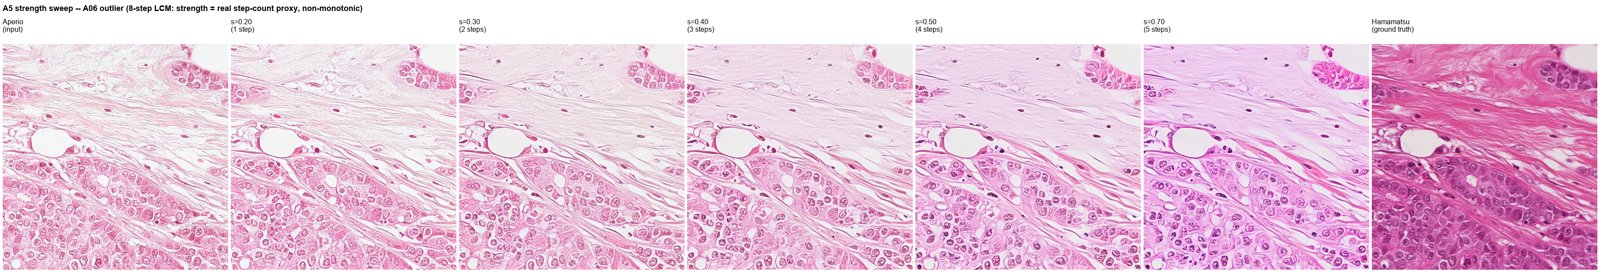
\includegraphics[width=\textwidth]{sweep_a5_06.jpg}\\[2pt]
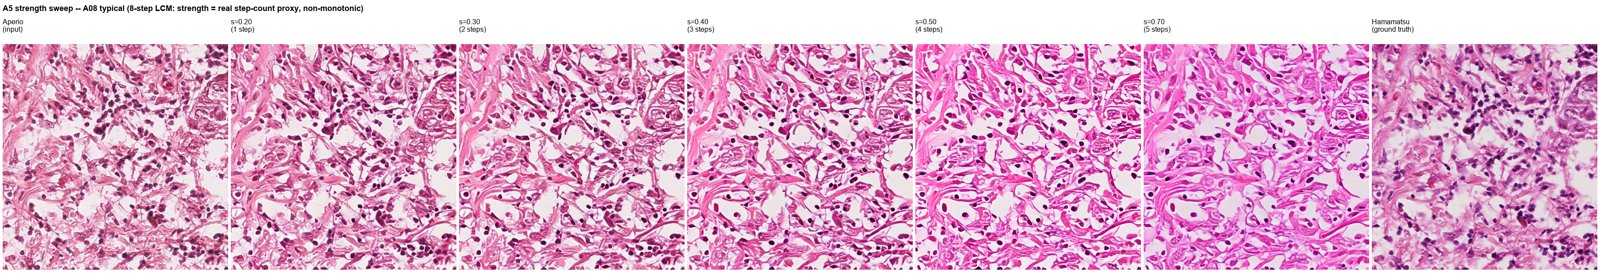
\includegraphics[width=\textwidth]{sweep_a5_08.jpg}
\caption{A5 strength sweep with 8 LCM steps on A06 (top) and A08 (bottom). Strength only sets how many steps
run ($\lfloor 8s\rfloor$). Colour moves towards the target on A06 as strength rises, while the typical slide
A08 loses both colour fidelity and structure.}
\label{fig:app-sweep}
\end{figure}

\begin{figure}[!htbp]
\centering
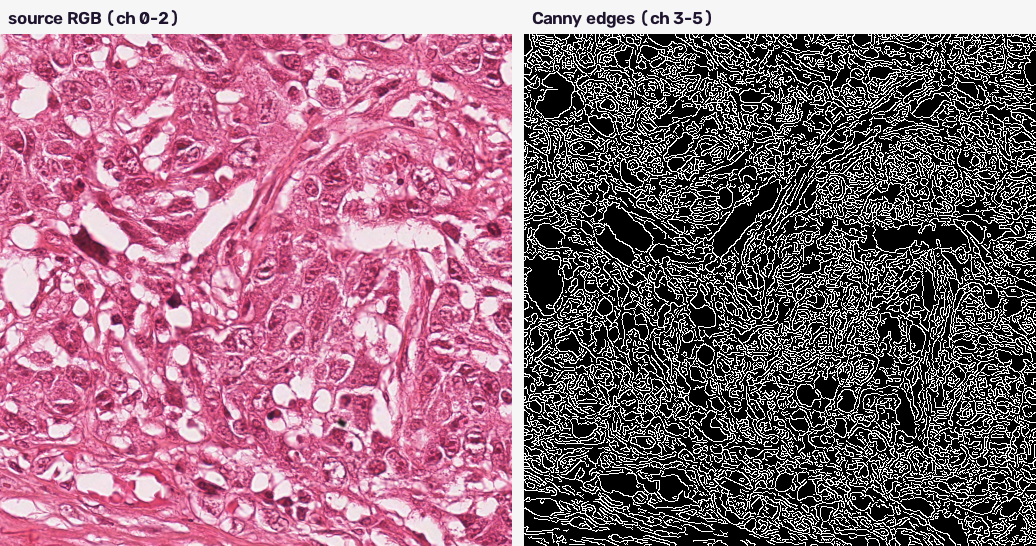
\includegraphics[width=0.42\textwidth]{controlnet_input.png}\hfill
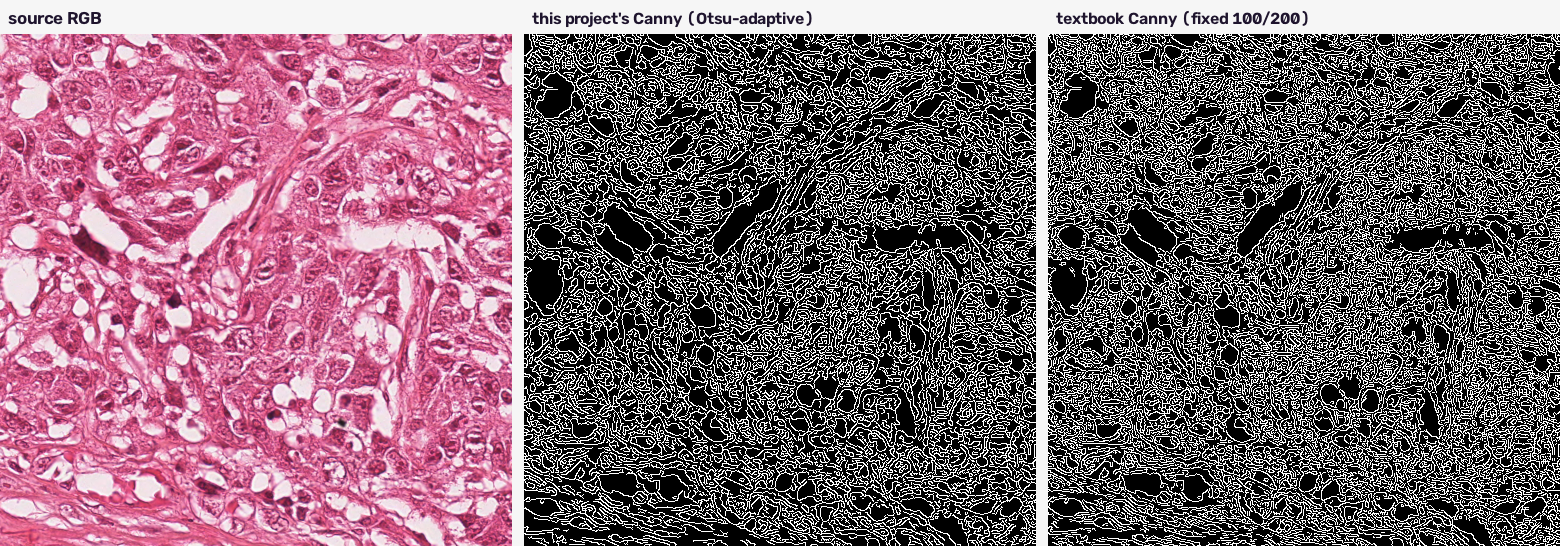
\includegraphics[width=0.56\textwidth]{controlnet_canny_comparison.png}
\caption{What the source-conditioned ControlNet sees (training crop A03\_00A). Left: the six-channel input,
source RGB and its Canny edges. Right: the source with our Otsu-adaptive Canny threshold and a fixed 100/200
threshold. Dense H\&E gives a busy edge map either way; the source RGB is the signal that lets the model learn
$p(H\mid A)$.}
\label{fig:app-controlnet}
\end{figure}

\begin{figure}[!htbp]
\centering
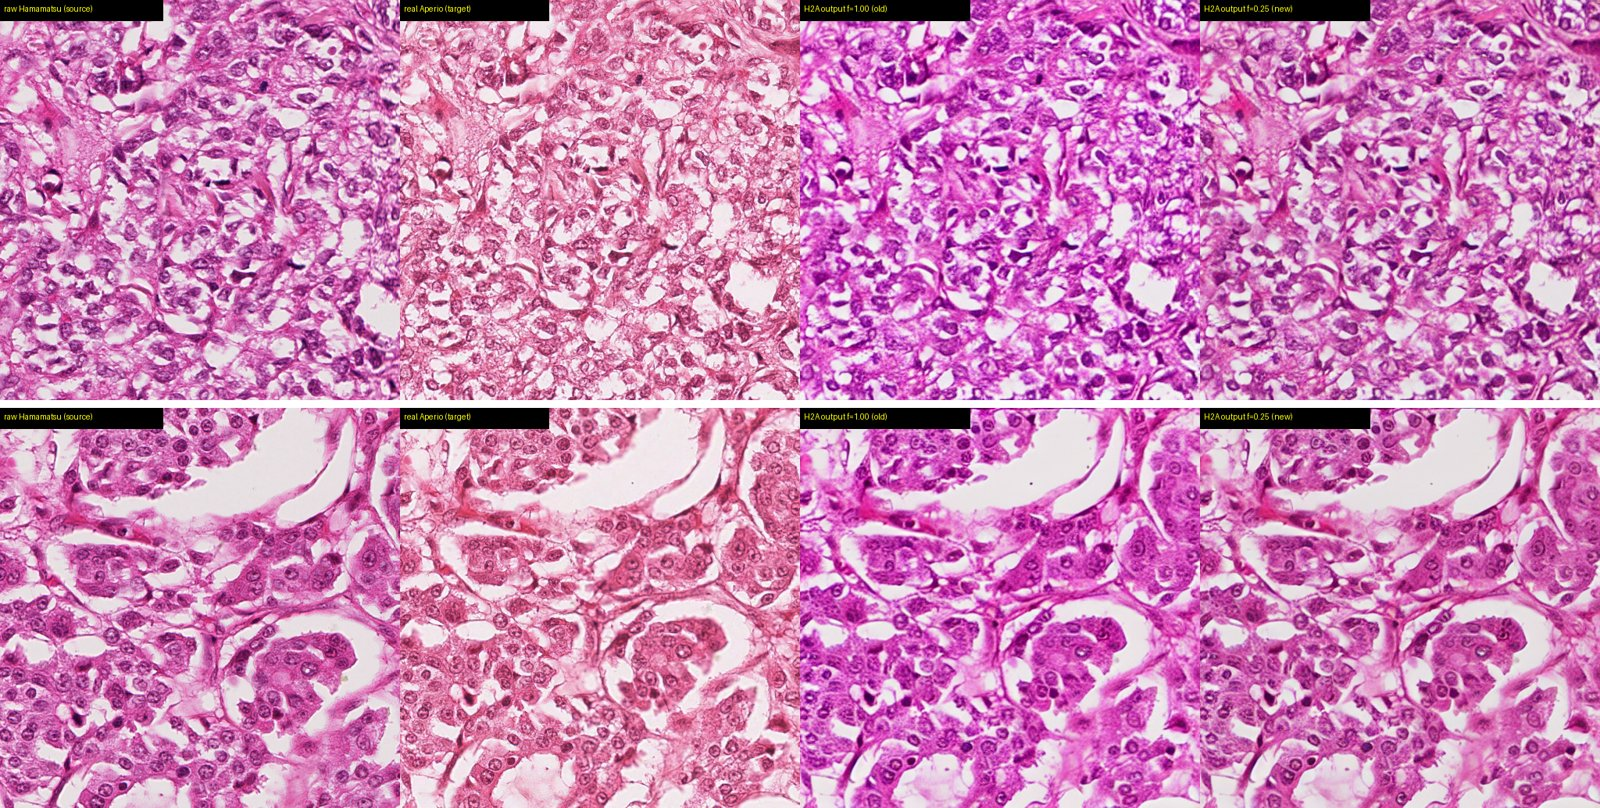
\includegraphics[width=0.72\textwidth]{p1_11_h2a.jpg}
\caption{SD\,1.5 in the \HtoA{} direction on held-out crops from A08 (top) and A16 (bottom): raw Hamamatsu source, real Aperio target,
and DDIM-inversion outputs with inversion fraction $f=1.00$ and $f=0.25$. Both drift towards magenta instead
of the paler Aperio colour ($\dlab=-15.6$ and $-6.2$).}
\label{fig:app-h2a}
\end{figure}

\begin{figure}[!htbp]
\centering
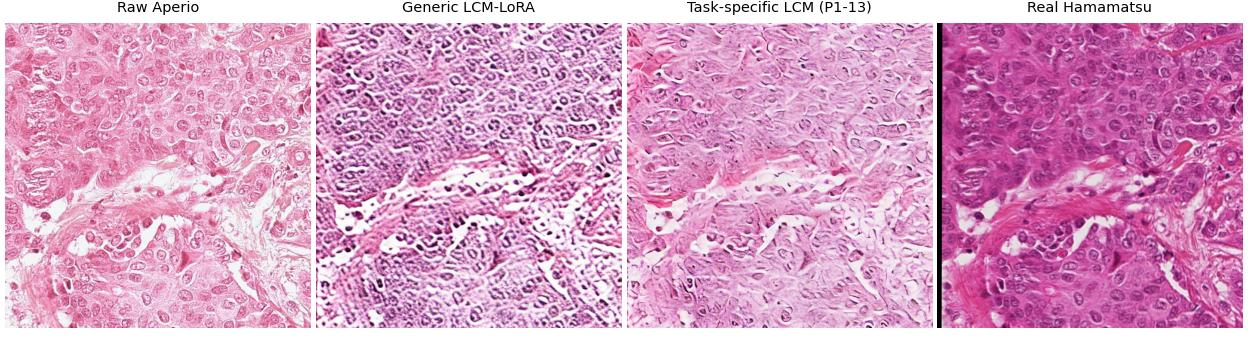
\includegraphics[width=0.8\textwidth]{p1_13_lcm.jpg}
\caption{Few-step inference on A06 (crop origin (0,0), seed 0): raw source, generic LCM-LoRA, the
task-specific distilled LCM, and the registered Hamamatsu target. Distillation did not improve on the generic
adapter.}
\label{fig:app-lcm}
\end{figure}

\begin{figure}[!htbp]
\centering
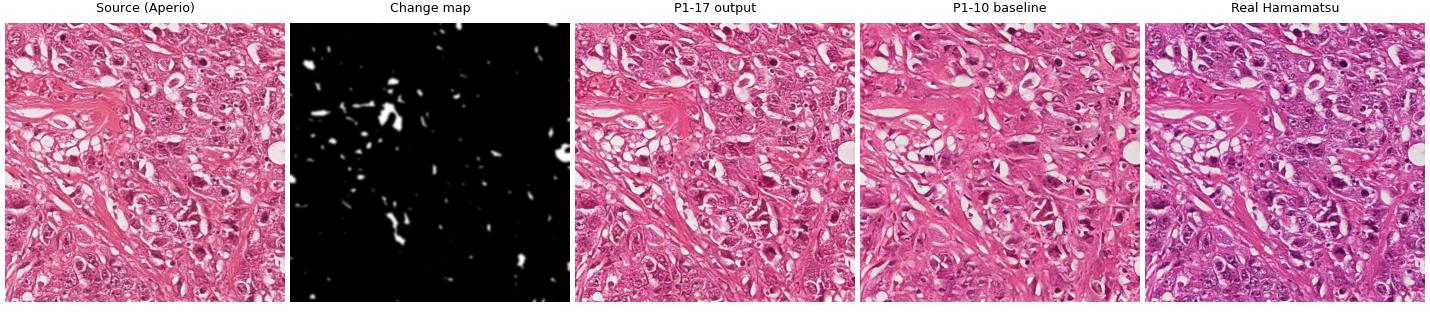
\includegraphics[width=0.9\textwidth]{p1_17_diffdiff.jpg}
\caption{Differential diffusion, a closed negative (training crop A03\_00A\_c024): source, the per-pixel change
map derived from edges, the differential-diffusion output, the plain source-conditioned baseline and the real
Hamamatsu crop. On dense H\&E the protected region covers nearly the whole crop, and SSIM did not change
(0.162--0.167 against $0.162\pm0.006$).}
\label{fig:app-diffdiff}
\end{figure}

\begin{figure}[!htbp]
\centering
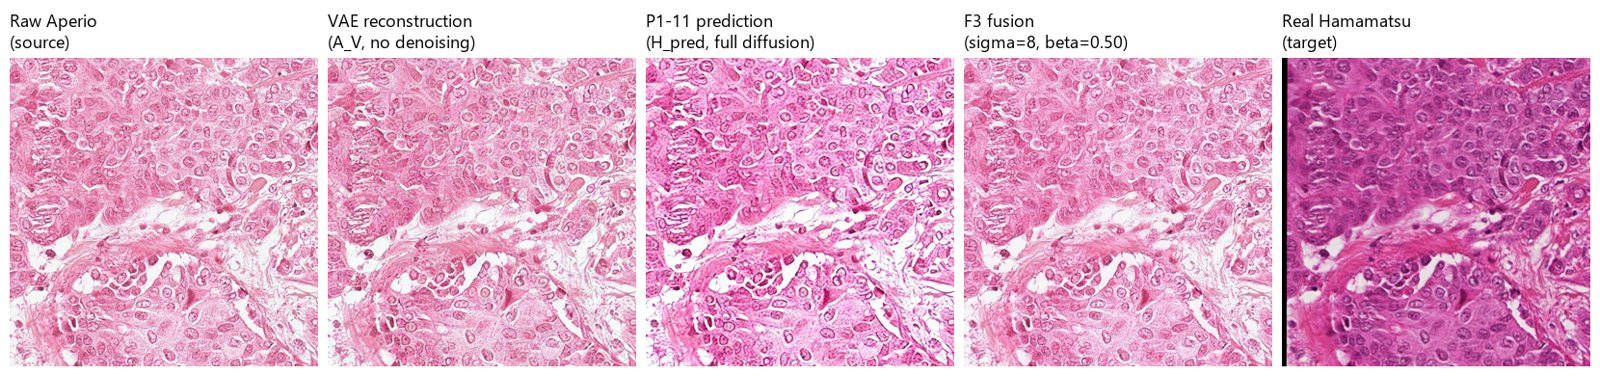
\includegraphics[width=\textwidth]{p1_16_a06.jpg}
\caption{F3 fusion on the outlier slide A06, laid out as Fig.~\ref{fig:f3}. The fused output keeps the source
structure but stays much paler than the Hamamatsu scan.}
\label{fig:app-f3}
\end{figure}

\begin{figure}[!htbp]
\centering
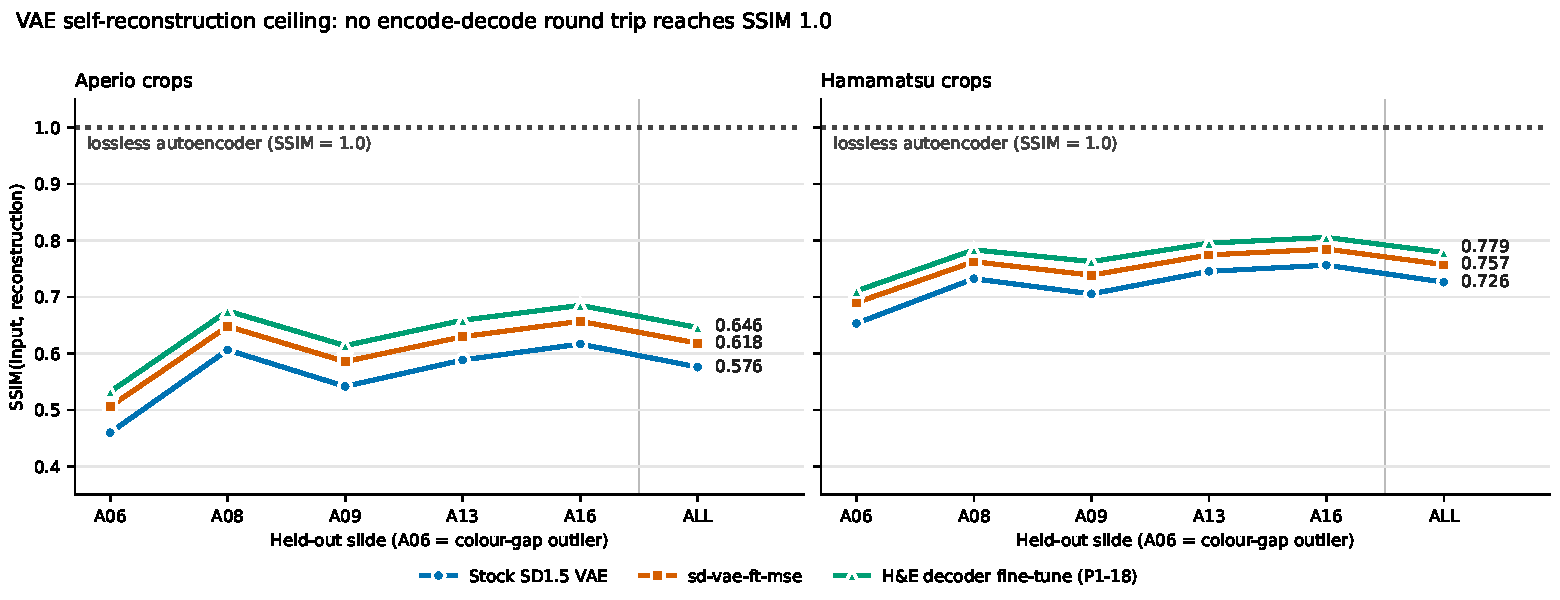
\includegraphics[width=0.9\textwidth]{vae_ceiling.pdf}
\caption{VAE self-reconstruction SSIM per held-out slide on Aperio (left) and Hamamatsu (right) crops, 496
crops each. The fine-tuned decoder is highest on every slide and every decoder stays far below the lossless
line (dotted).}
\label{fig:app-vae}
\end{figure}

\begin{figure}[!htbp]
\centering
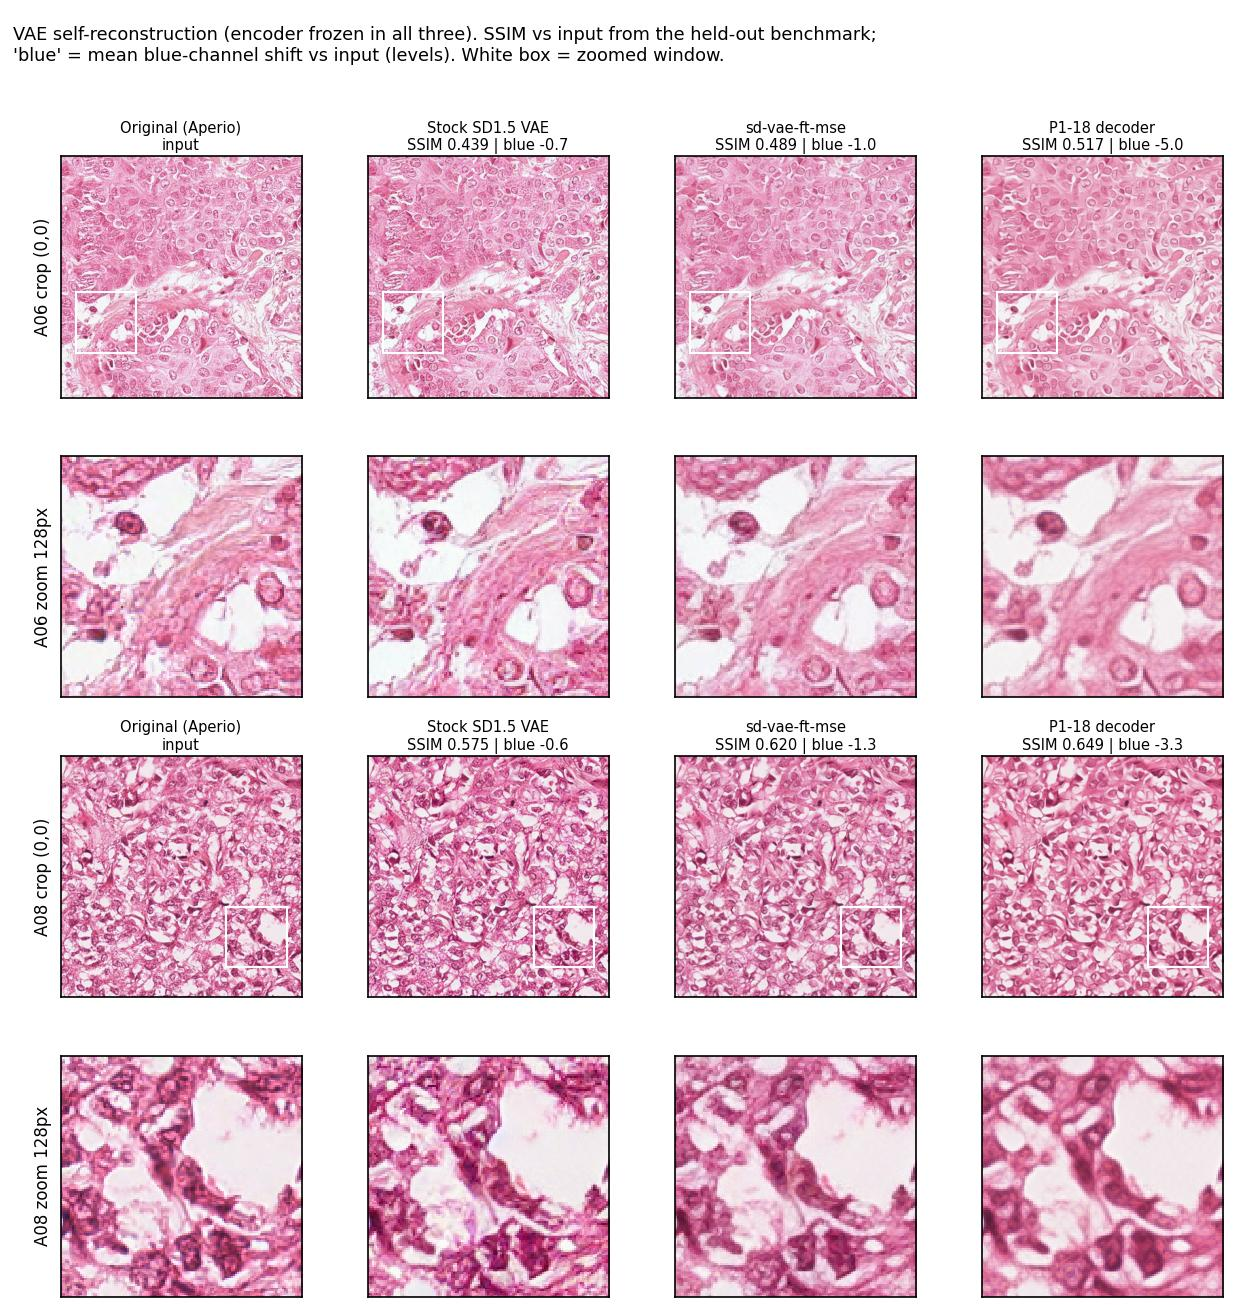
\includegraphics[width=0.47\textwidth]{p1_18_g12_recon.jpg}\hfill
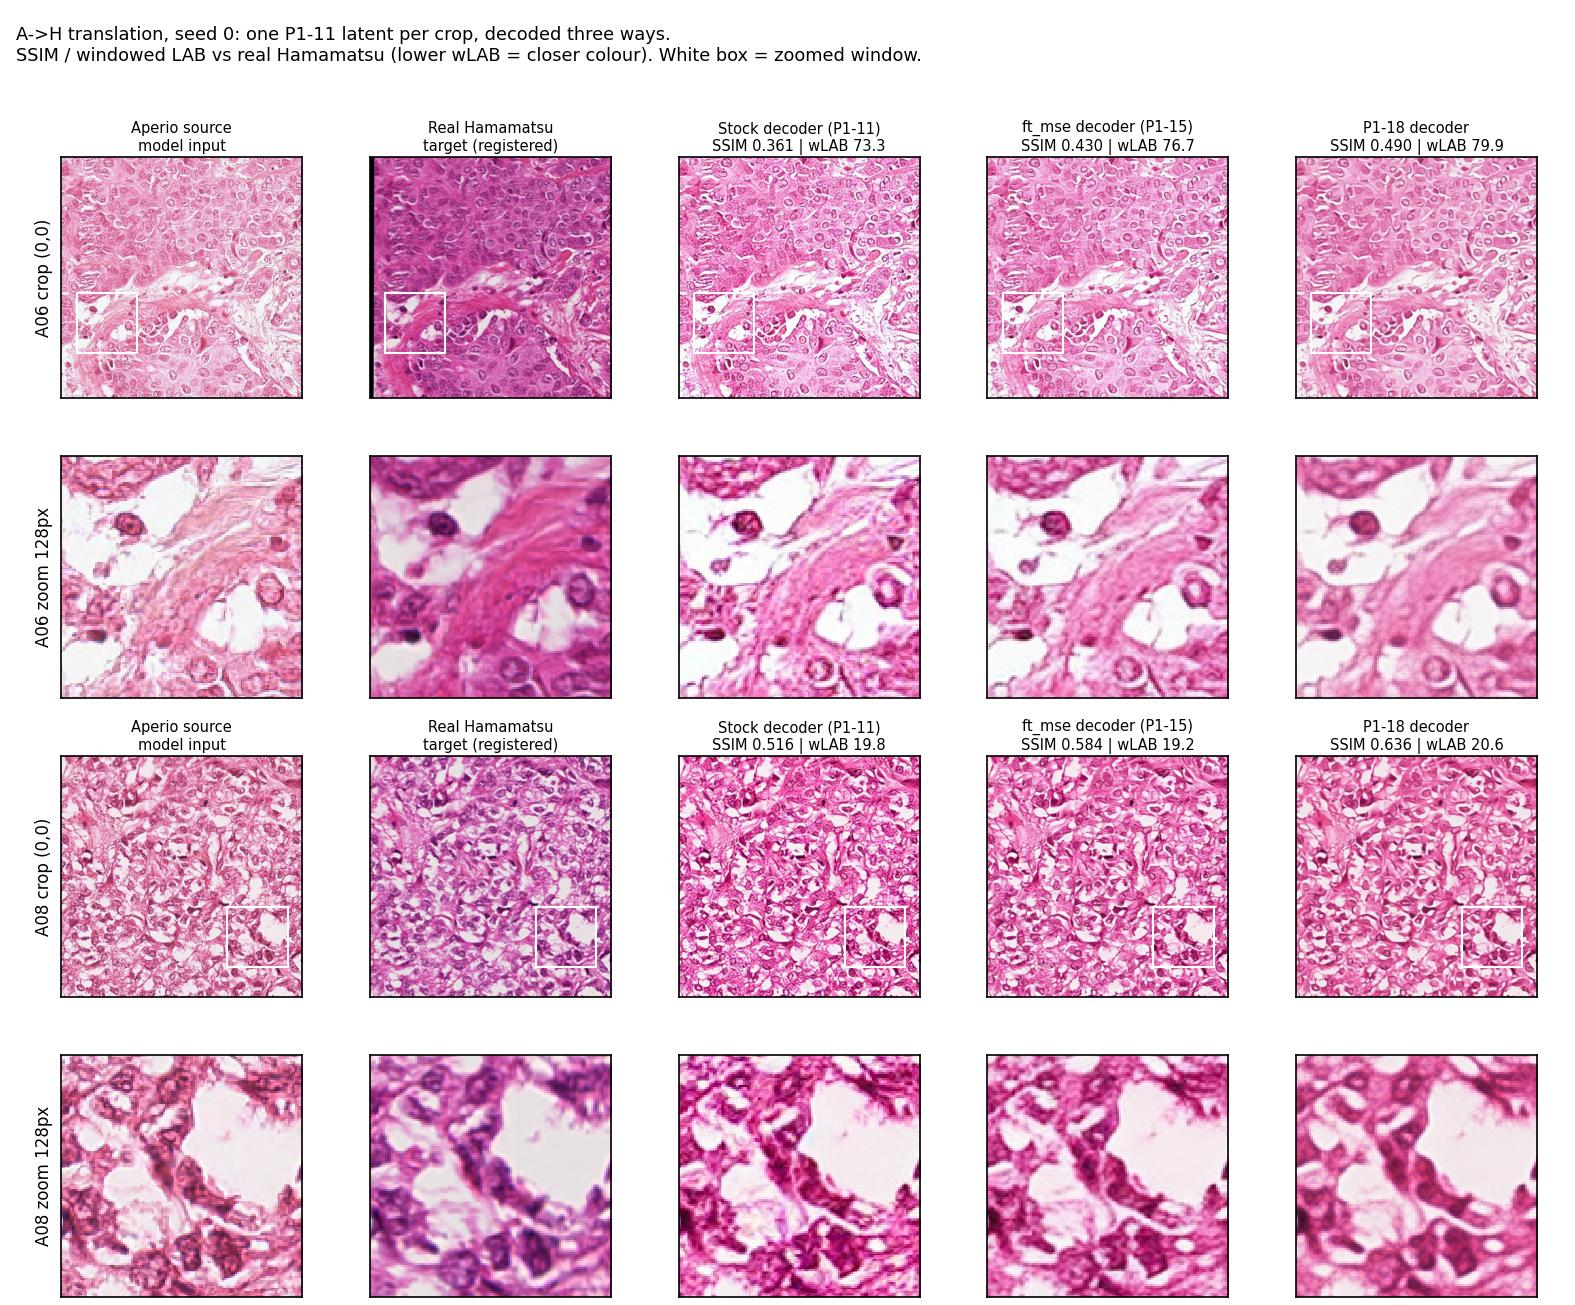
\includegraphics[width=0.52\textwidth]{p1_18_g12_translated.jpg}
\caption{Decoder comparison on A06 and A08, each with a 128\,px zoom. Left: self-reconstruction by the stock,
\texttt{ft-mse} and fine-tuned decoders, with SSIM and blue-channel shift against the input. Right: the same
DDIM-inversion latent decoded three ways, with SSIM and windowed LAB against the real Hamamatsu scan. The
fine-tuned decoder is the smoothest, which raises SSIM against the soft Hamamatsu target, and it shifts
colour slightly towards pink.}
\label{fig:app-decoder}
\end{figure}

\begin{figure}[!htbp]
\centering
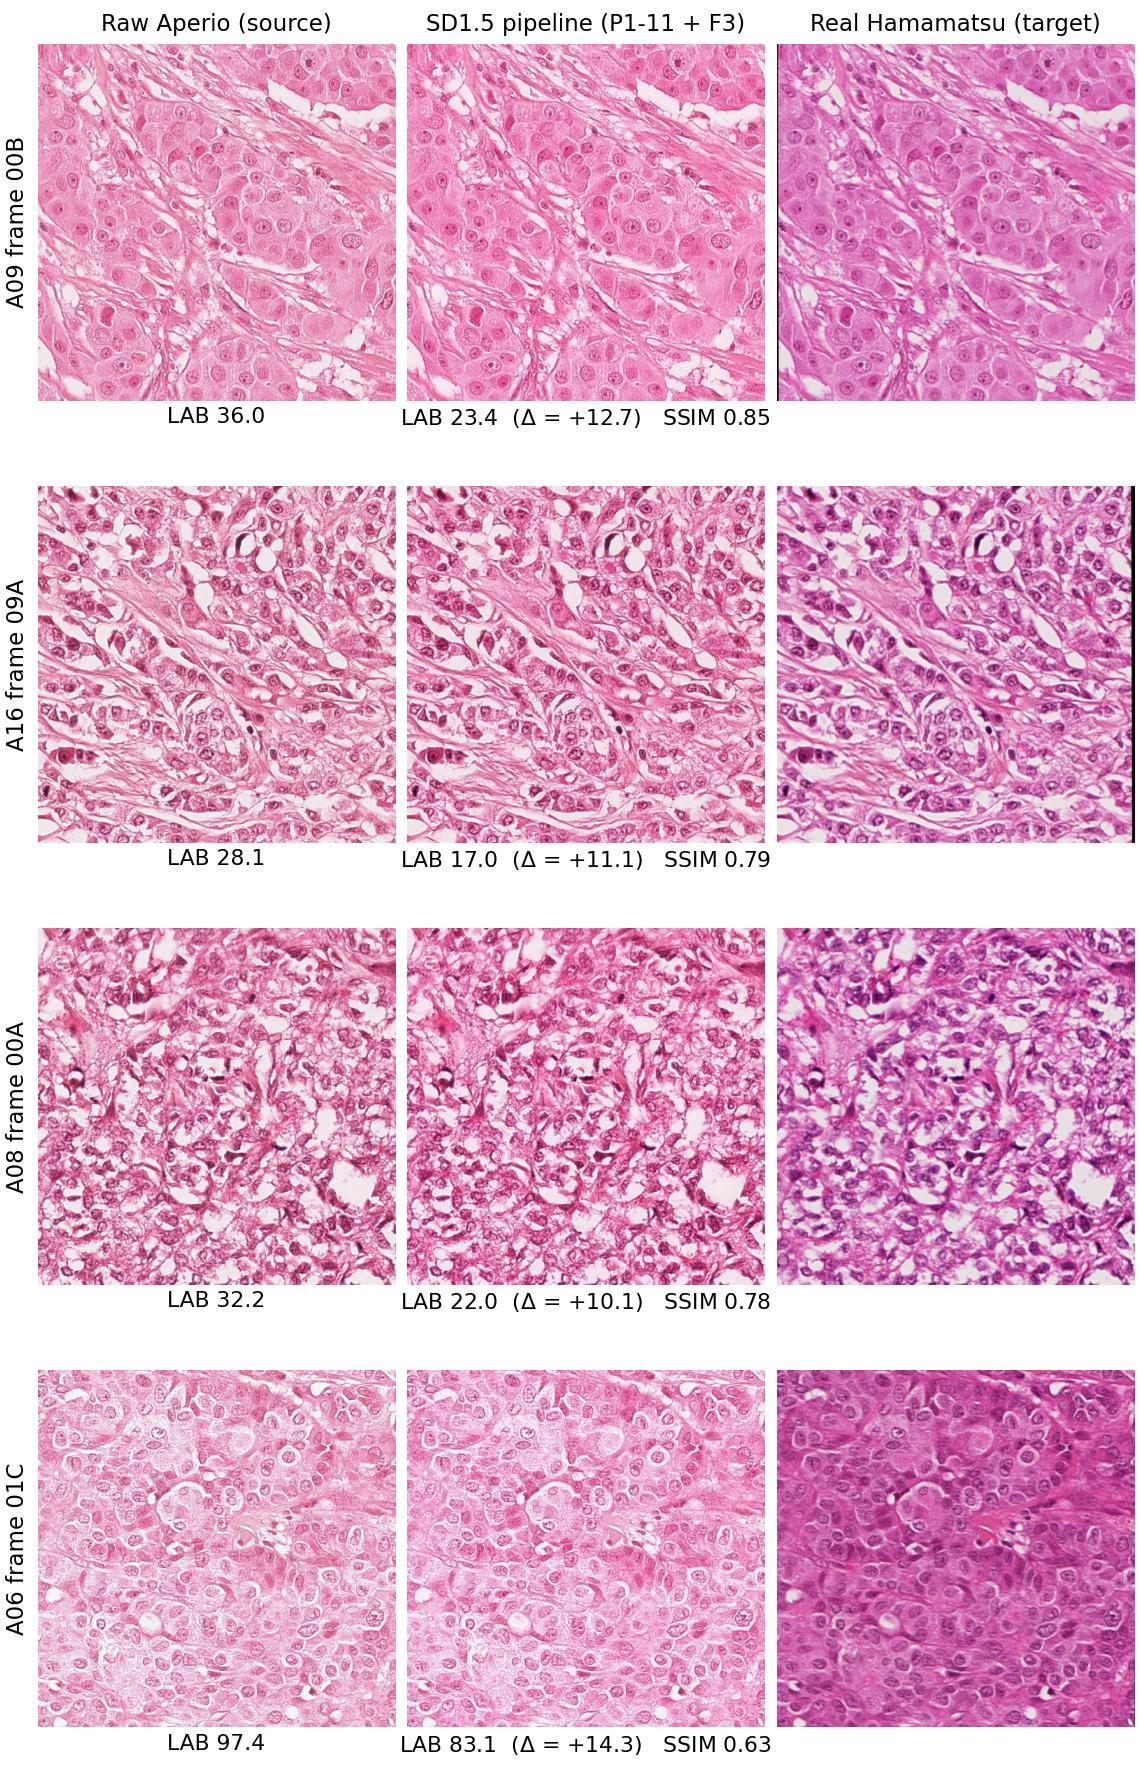
\includegraphics[width=0.46\textwidth]{best_cases_sd15.jpg}
\caption{Selected best cases of the final SD\,1.5 pipeline (DDIM inversion + F3 fusion): the top crop by
recovery on A09, A16, A08 and A06, with raw source, output and registered target. These are not typical: mean
recovery per slide is $+7.2$ to $+10.8$, and A06 stays paler than its target.}
\label{fig:app-best}
\end{figure}

\clearpage
\section{Evaluation figures}
\label{app:eval}

\begin{figure}[!htbp]
\centering
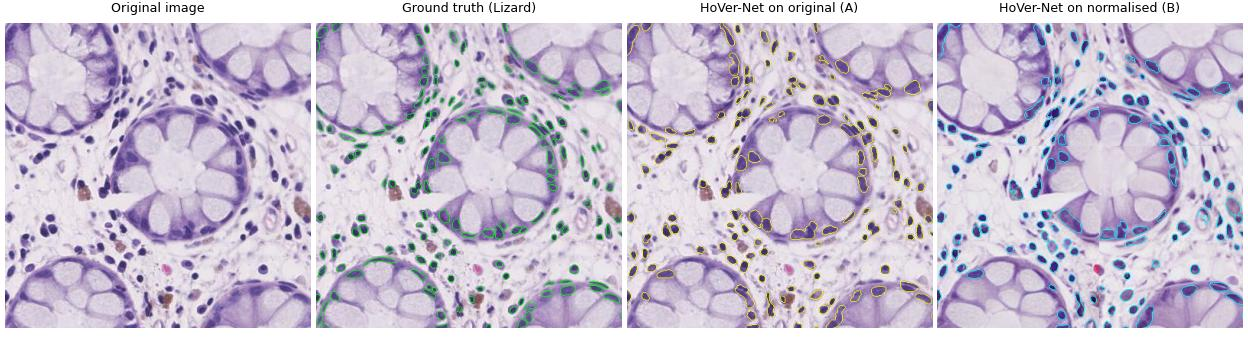
\includegraphics[width=0.8\textwidth]{lizard_overlay.jpg}
\caption{Structural-safety test on a typical Lizard image (400\,px patch; Dice(A,G) 0.741, Dice(B,G) 0.651,
ratio 0.878, the median): original, ground-truth nuclei, HoVer-Net on the original and on the normalised
image. HoVer-Net finds fewer nuclei after normalisation.}
\label{fig:app-lizard}
\end{figure}

\begin{figure}[!htbp]
\centering
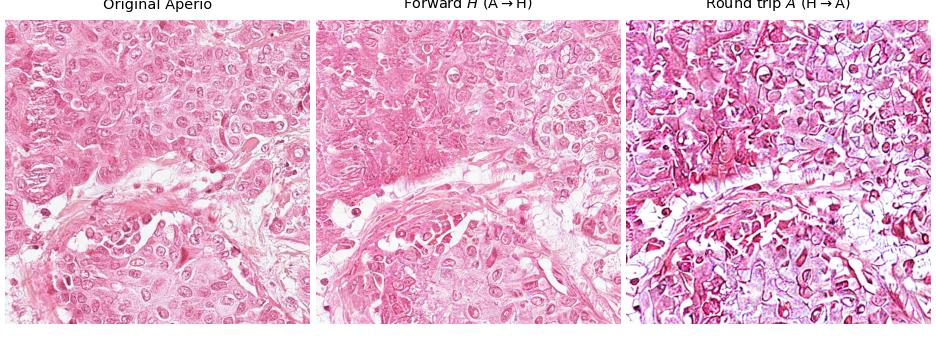
\includegraphics[width=0.62\textwidth]{roundtrip.jpg}
\caption{Round trip \AtoH{}\,$\to$\,A on A06 (50-step DDIM, strength 0.20): original, forward output and the
return trip. The return is oversaturated with distorted nuclear detail (SSIM 0.143 over 64 crops).}
\label{fig:app-roundtrip}
\end{figure}

\begin{figure}[!htbp]
\centering
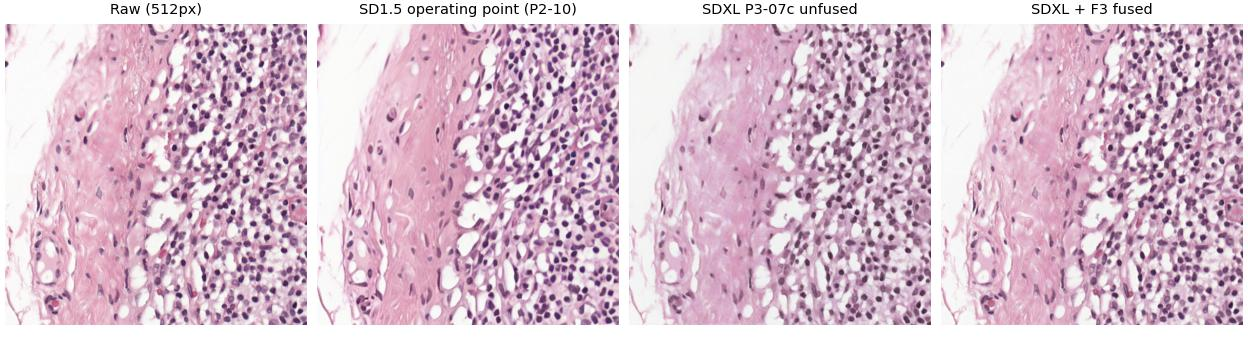
\includegraphics[width=0.85\textwidth]{camelyon_sdxl.jpg}
\caption{CAMELYON17 centre~0: raw patch, the SD\,1.5 operating-point output (the failed cross-centre test), and
the 144-pair SDXL model, unfused and with F3 fusion (run at 1024\,px).}
\label{fig:app-camelyon}
\end{figure}

\clearpage
\section{SDXL and probe figures}
\label{app:sdxl}

\begin{figure}[!htbp]
\centering
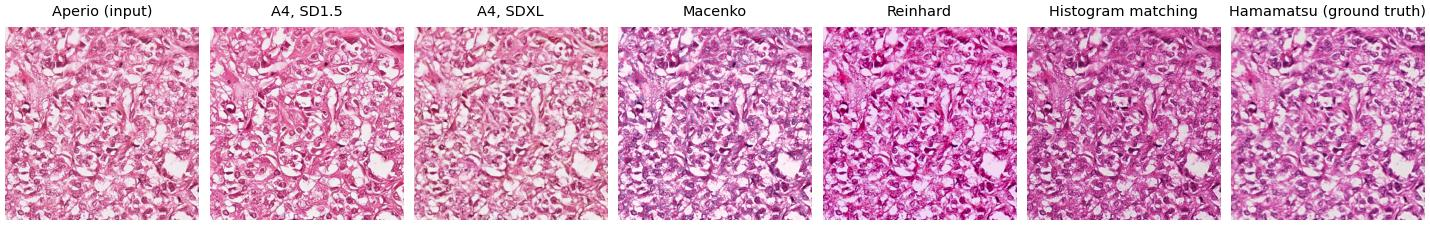
\includegraphics[width=\textwidth]{sdxl_vs_sd15.jpg}
\caption{A08 at the A4 configuration (strength 0.20) on SD\,1.5 and SDXL, with the classical baselines and the
real Hamamatsu scan.}
\label{fig:app-sdxl-sd15}
\end{figure}

\begin{figure}[!htbp]
\centering
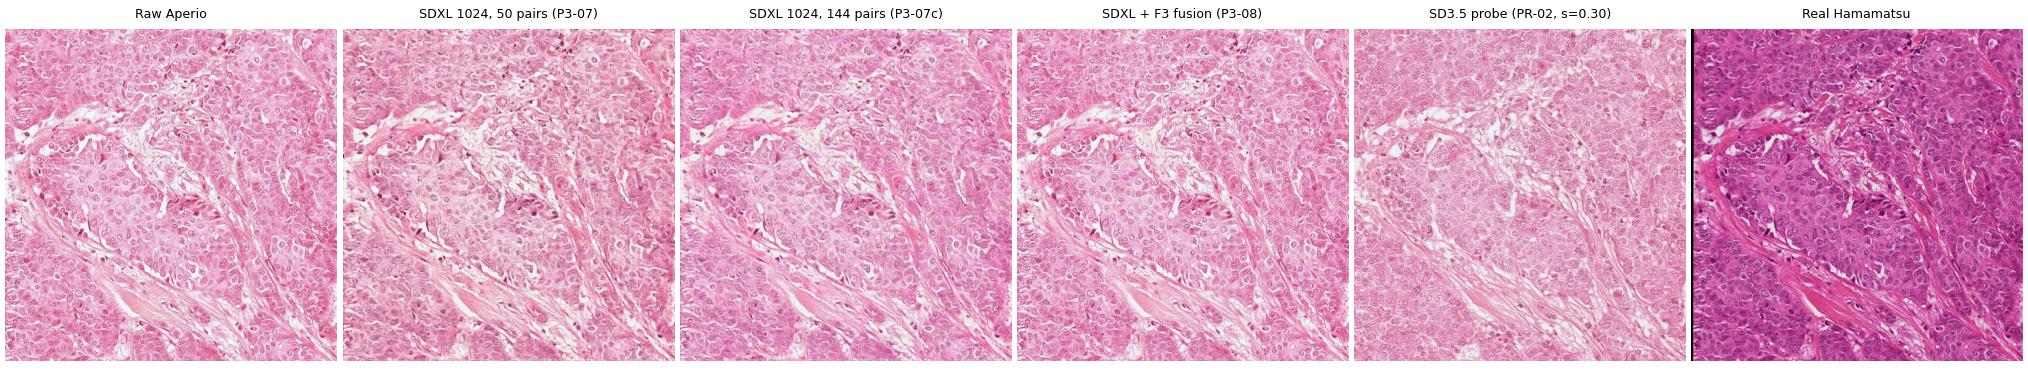
\includegraphics[width=\textwidth]{sdxl_sd35_panel_a06.jpg}
\caption{One 1024\,px A06 crop across methods, including the SD\,3.5 probe output (strength 0.30). The 50-pair
SDXL output stays near the Aperio colour, the 144-pair output is slightly more saturated, F3 fusion restores
source detail, and SD\,3.5 is washed out. The black strip on the Hamamatsu tile is registration padding.}
\label{fig:app-sd35}
\end{figure}

\begin{figure}[!htbp]
\centering
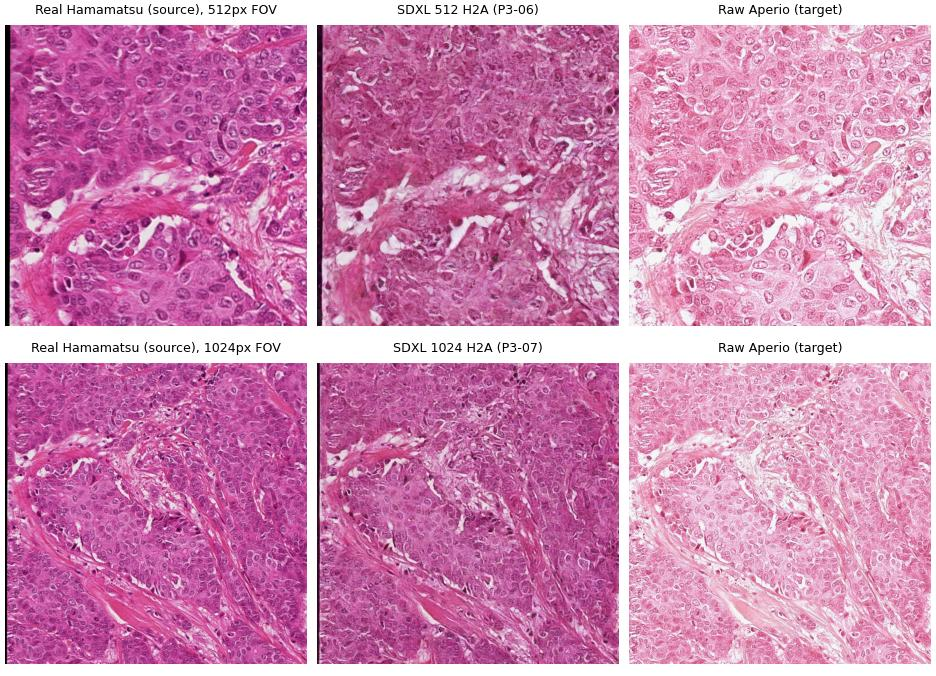
\includegraphics[width=0.6\textwidth]{sdxl_h2a.jpg}
\caption{SDXL \HtoA{} on A06 at 512\,px (top) and 1024\,px (bottom): real Hamamatsu source, SDXL output and raw
Aperio target. On this crop both outputs stay closer to the source than to the pale target; the mean
recoveries are $+9.47$ and $+9.20$.}
\label{fig:app-sdxl-h2a}
\end{figure}

\begin{figure}[!htbp]
\centering
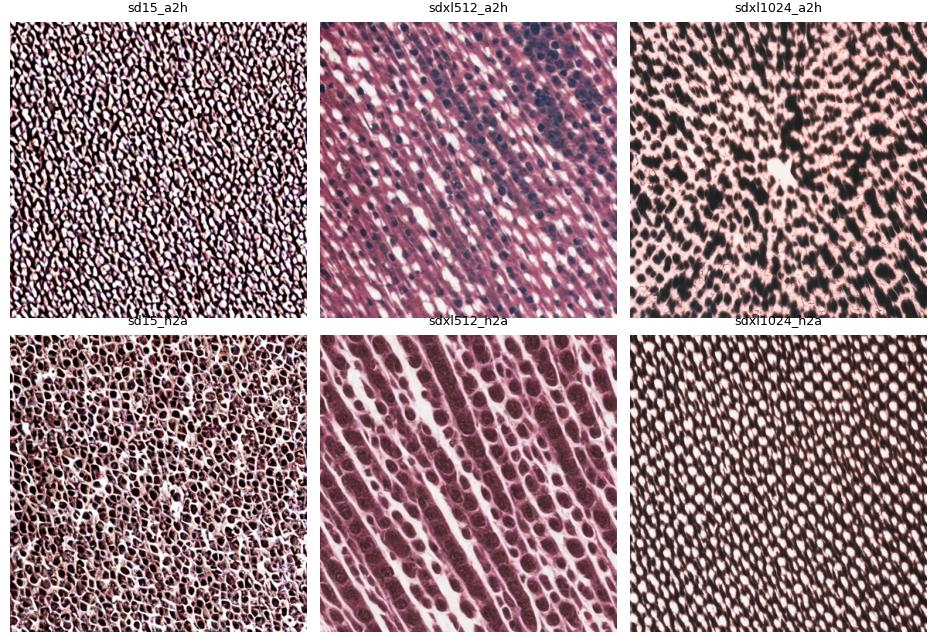
\includegraphics[width=0.6\textwidth]{t2i_backbones.jpg}
\caption{Pure text-to-image samples (seed 0) from SD\,1.5, SDXL at 512\,px and SDXL at 1024\,px, used only to
read each backbone's default colour in a diagnostic of the \AtoH{}/\HtoA{} asymmetry. They are repetitive
textures, not realistic tissue.}
\label{fig:app-t2i}
\end{figure}

\begin{figure}[!htbp]
\centering
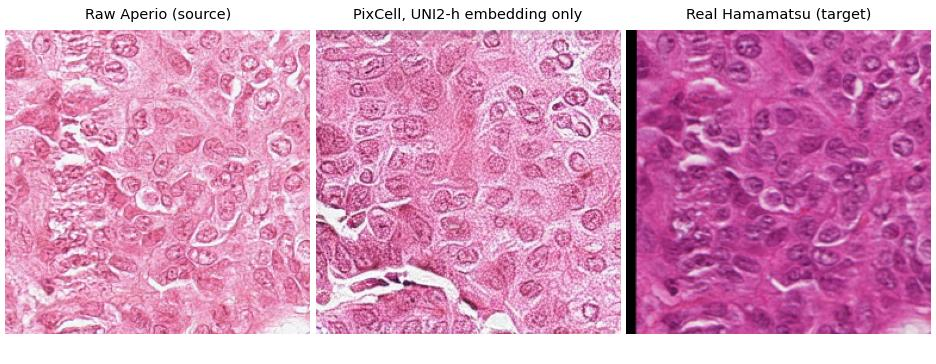
\includegraphics[width=0.62\textwidth]{pixcell_floor.jpg}
\caption{PixCell generation without fine-tuning from the crop's own UNI2-h embedding (A06, frame 00A, 256\,px).
The output is plausible H\&E tissue, but nuclei and glands are not where they are in the source or target
(SSIM 0.045).}
\label{fig:app-pixcell}
\end{figure}


\end{document}
